\label{introducao}

A adoção crescente de sistemas baseados em IA tem transformado significativamente a forma como soluções tecnológicas são concebidas e desenvolvidas. Esse avanço, contudo, vem acompanhado por um aumento relevante das preocupações éticas, especialmente no que diz respeito à transparência, equidade, responsabilidade, explicabilidade e privacidade \cite{Floridi2018, Jobin2019, Ryan2020}. Casos documentados de vieses algorítmicos, decisões automatizadas discriminatórias e uso indevido de dados sensíveis indicam a necessidade de incorporar princípios éticos em todas as etapas do desenvolvimento de software \cite{Mittelstadt2019, Hagendorff2020, Obermeyer2019}.

A popularização de sistemas baseados em IA trouxe consigo uma série de incidentes de grande visibilidade, evidenciando lacunas na operacionalização de princípios éticos. Entre os casos mais significativos, destaca-se o estudo de Obermeyer et al. \cite{Obermeyer2019}, publicado na revista \textit{Science}, que documentou como um algoritmo comercial usado para gerenciar o cuidado de aproximadamente 70 milhões de pacientes nos Estados Unidos apresentava viés racial sistemático. O sistema utilizava custos de saúde como \textit{proxy} para necessidades médicas, resultando em pacientes negros sendo 26\% mais doentes que pacientes brancos com a mesma pontuação de risco. Esse viés reduziu drasticamente a inscrição de pacientes negros em programas de cuidado, de 46,5\% para 17,7\%.

No domínio de reconhecimento facial, o estudo \textit{Gender Shades} conduzido por Buolamwini \& Gebru \cite{Buolamwini2018} revelou disparidades interseccionais significativas em sistemas comerciais de classificação de gênero. A pesquisa demonstrou taxas de erro de até 34,7\% para mulheres de pele escura, comparadas a apenas 0,8\% para homens de pele clara. Esse trabalho catalisou mudanças na indústria, levando empresas como IBM e Microsoft a aprimorarem seus sistemas e a Amazon a descontinuar o uso de tecnologias de reconhecimento facial para aplicações de segurança pública.

Mais recentemente, no contexto de sistemas de contratação, Sheard \cite{Sheard2025} documentou discriminação algorítmica contra mulheres, trabalhadores mais velhos e pessoas com deficiência em plataformas como HireVue e Sapia. A pesquisa identificou taxas de erro de transcrição de 22\% para falantes não-nativos de inglês, comparadas a 5-10\% em transcrições humanas. Em 2023, a empresa iTutorGroup foi condenada pela \textit{Equal Employment Opportunity Commission} (EEOC) dos Estados Unidos a pagar 365 mil dólares em acordo por discriminação etária facilitada por algoritmos.

Esses problemas estão diretamente relacionados à operacionalização dos princípios éticos de IA. Os casos documentados em sistemas de saúde, reconhecimento facial e contratação poderiam ter sido evitados ou mitigados se princípios como transparência (\textit{transparency}), justiça (\textit{fairness}), responsabilidade (\textit{accountability}), explicabilidade (\textit{explainability}) e não-maleficência (\textit{non-maleficence}) tivessem sido sistematicamente verificados durante o processo de desenvolvimento. Portanto, é fundamental que o desenvolvimento de sistemas de IA seja orientado por uma estrutura ética robusta que não apenas antecipe os possíveis impactos negativos, mas também forneça mecanismos automatizados para sua detecção e prevenção.

Com isso, a fim de prevenir novos incidentes e garantir a conformidade ética de sistemas de IA, diversas diretrizes e princípios éticos foram propostas nos últimos anos \cite{UNESCO2021, EUAIAct2024}. A análise de Jobin et al. \cite{Jobin2019} de 84 documentos contendo princípios ou diretrizes éticas para IA, identificou convergências globais em torno de princípios como transparência, justiça, responsabilidade, privacidade e explicabilidade. Mais recentemente, Corrêa et al. \cite{Corrêa2023} expandiram essa análise para 200 diretrizes globais, identificando 17 princípios éticos prevalentes. No entanto, mesmo com o crescente número de pesquisas e regulamentações, ainda há falta de consenso quanto à definição operacional de "IA ética" e, principalmente, quanto aos requisitos técnicos necessários para sua implementação \cite{Ryan2020}.

Uma dificuldade significativa identificada na literatura é que os princípios éticos propostos são, em sua maioria, abstratos e gerais, não constituindo soluções práticas que possam ser integradas ao ciclo de vida do desenvolvimento de software \cite{Mittelstadt2019, Hagendorff2020}. O estudo de Vakkuri et al. \cite{S012}, que propõe o método ECCOLA para implementação de sistemas de IA eticamente alinhados, identificou que as diretrizes existentes permanecem predominantemente em um nível teórico, não oferecendo métodos operacionalizáveis para detecção e prevenção de falhas éticas durante o desenvolvimento. Morley et al. \cite{Morley2020} conduziram uma revisão inicial de ferramentas, métodos e pesquisas disponíveis publicamente para traduzir princípios em práticas, identificando que existe uma lacuna significativa entre os aspectos conceituais e a implementação prática de ética em IA.

Outra lacuna relevante é a ausência de ferramentas automatizadas para avaliar e detectar violações éticas em modelos de IA já implementados. Enquanto técnicas de teste de software tradicionais focam em requisitos funcionais e não-funcionais como desempenho e segurança, há uma carência de abordagens sistemáticas para testar conformidade ética. O trabalho de Holstein et al. \cite{Holstein2019} identificou que profissionais de IA enfrentam desafios significativos nos processos de avaliação de \textit{fairness}, incluindo dificuldades em definir métricas apropriadas, obter dados adequados para testes e interpretar resultados em contextos específicos de aplicação.

Técnicas de \textit{fuzzing}, tradicionalmente utilizadas para detectar vulnerabilidades de segurança em software, podem ser adaptadas para identificar falhas éticas em modelos de IA. O trabalho de Zhang et al. \cite{Zhang2019} demonstra que é possível operacionalizar princípios éticos abstratos em testes automatizados, permitindo a detecção sistemática de vieses, falta de transparência e problemas de \textit{accountability} em modelos de linguagem e outros sistemas de IA. No entanto, essa abordagem ainda está em estágio inicial e requer desenvolvimento de ferramentas práticas e modulares que possam ser integradas a processos de desenvolvimento de software.

Para fundamentar a seleção de princípios éticos prioritários a serem operacionalizados neste trabalho, foi conduzido um Mapeamento Sistemático da Literatura (MSL), apresentado no Capítulo~\ref{cap:rsl}. O mapeamento seguiu as diretrizes metodológicas de Petersen et al. \cite{Petersen2015} e analisou 58 estudos primários publicados entre 2020 e 2025, identificando quais princípios éticos são mais abordados pela literatura sobre ética aplicada a sistemas de IA no contexto da Engenharia de Software (RQ1) e quais abordagens são propostas para operacionalizar esses princípios ao longo do ciclo de vida do software (RQ2).

Os resultados do mapeamento sistemático revelaram três princípios éticos predominantes na literatura: \textit{Fairness} foi identificado em 82,8\% dos estudos (48 de 58), \textit{Accountability} em 55,2\% (32 de 58) e \textit{Transparency} em 50,0\% (29 de 58). Esses três princípios não apenas são os mais discutidos conceitualmente, mas também apresentam o maior número de abordagens de operacionalização propostas, incluindo métodos, \textit{frameworks}, ferramentas e artefatos aplicáveis às diferentes fases do ciclo de vida de desenvolvimento de software (SDLC).

A análise das abordagens de operacionalização (RQ2) demonstrou que as contribuições existentes concentram-se principalmente nas fases de \textit{Requirements} (55,2\% dos estudos), \textit{Design} (50,0\%) e \textit{Implementation} (56,9\%), enquanto a fase de \textit{Testing} é abordada em apenas 37,9\% dos estudos. Essa lacuna é particularmente significativa, considerando que testes automatizados são essenciais para verificar conformidade ética de forma sistemática e escalável. Os estudos identificados na fase de \textit{Testing} propõem principalmente conjuntos de testes de \textit{fairness}, critérios de cobertura sensível a grupos protegidos e procedimentos de validação de desempenho diferencial entre grupos. No entanto, essas práticas ainda são aplicadas predominantemente em contextos experimentais, com relativamente pouca evidência de adoção sistemática em ambientes de desenvolvimento contínuo.

Assim, este trabalho propõe o desenvolvimento de \textit{fuzzing engines} automatizadas para apoiar a operacionalização dos princípios éticos de Transparência (\textit{Transparency}), Justiça (\textit{Fairness}) e Responsabilidade (\textit{Accountability}) em modelos de IA. A seleção desses três princípios é fundamentada nos resultados do mapeamento sistemático conduzido, que os identifica como os mais prevalentes na literatura (82,8\%, 55,2\% e 50,0\%, respectivamente) e como aqueles que apresentam maior maturidade em termos de abordagens de operacionalização propostas. As \textit{fuzzing engines} desenvolvidas funcionarão como componentes modulares, integradas a um sistema completo de \textit{fuzzing} ético, permitindo que desenvolvedores testem seus modelos de IA quanto a conformidade ética de forma sistemática e automatizada.

\section{Justificativa}

A necessidade de ética em IA decorre dos desafios encontrados em equilibrar a tensão entre o apoio à inovação tecnológica e a limitação dos possíveis danos associados a sistemas baseados em IA mal projetados ou não testados adequadamente \cite{Morley2020}. Portanto, é de grande importância desenvolver soluções práticas que permitam a verificação sistemática de conformidade ética durante o desenvolvimento e operação de sistemas de IA.

O trabalho de Birhane et al. \cite{Birhane2022}, vencedor do prêmio Distinguished Paper na conferência ACM FAccT 2022, analisou 100 artigos altamente citados de conferências de \textit{machine learning} (ICML e NeurIPS) e identificou que apenas 16\% dos trabalhos justificam conexão com necessidades sociais reais, e apenas 1\% discute potenciais impactos negativos de suas contribuições. Essa lacuna entre desenvolvimento técnico e considerações éticas reforça a necessidade de ferramentas que auxiliem desenvolvedores a incorporar princípios éticos de forma prática e verificável.

O mapeamento sistemático conduzido neste trabalho (Capítulo~\ref{cap:rsl}) identificou seis lacunas principais na literatura sobre operacionalização de ética em IA no contexto da Engenharia de Software. Dentre essas lacunas, duas são particularmente relevantes para este trabalho:

\textbf{Lacuna 2 (L2) -- Suporte Ferramental Integrado:} A maioria das ferramentas propostas não se integra a ecossistemas reais como IDEs, \textit{pipelines} de CI/CD ou plataformas de MLOps. Há necessidade de soluções que funcionem dentro dos fluxos de desenvolvimento já adotados pela indústria \cite{S010, S021, S030}.

\textbf{Lacuna 4 (L4) -- \textit{Gap} Academia--Indústria:} Faltam evidências empíricas sobre adoção industrial. Poucos estudos apresentam casos reais, métricas de custo-benefício ou análises robustas de escalabilidade e sustentabilidade das abordagens \cite{Holstein2019}.

Além disso, a análise das fases do SDLC (RQ2) revelou que, embora a fase de \textit{Testing} seja crítica para garantir conformidade ética, apenas 37,9\% dos estudos (22 de 58) propõem abordagens específicas para essa fase. Os estudos existentes \cite{S003, S004, S022, S034} concentram-se principalmente em testes de \textit{fairness}, com menor cobertura de testes para \textit{transparency} e \textit{accountability}. Essa lacuna contrasta com a alta prevalência desses princípios na literatura (50,0\% e 55,2\%, respectivamente), indicando uma desconexão entre a discussão conceitual e a operacionalização prática em testes automatizados.

No contexto regulatório, a entrada em vigor do \textit{EU AI Act} \cite{EUAIAct2024} e a publicação de diretrizes por organizações como UNESCO \cite{UNESCO2021}, OECD e IEEE estabelecem requisitos legais e normativos para sistemas de IA em aplicações de alto risco. Esses marcos regulatórios exigem demonstração de conformidade com princípios éticos, incluindo transparência, justiça e responsabilidade. No entanto, os métodos atuais de auditoria são predominantemente manuais, custosos e não escaláveis \cite{S014}. O trabalho de Lam et al. \cite{Lam2024} propôs um \textit{framework} de auditorias de garantia para sistemas algorítmicos, modelado após práticas de auditoria financeira, mas reconhece que a automação desses processos ainda é um desafio em aberto.

A abordagem de \textit{Ethics by Design} proposta por Vakkuri et al. \cite{S012, S013} no método ECCOLA e adotada em diversos contextos de desenvolvimento de IA reforça a importância de integrar considerações éticas desde as fases iniciais do desenvolvimento. No entanto, a operacionalização desse modelo ainda carece de ferramentas automatizadas específicas para cada princípio ético, particularmente na fase de \textit{Testing}.

No contexto de testes de software, a literatura sobre \textit{fairness} em \textit{machine learning} \cite{Caton2024, Pessach2020} identifica que técnicas de mitigação de viés são aplicadas predominantemente em três momentos: pré-processamento (tratamento de dados), \textit{in-processing} (modificação de algoritmos) e pós-processamento (ajuste de predições). No entanto, há uma lacuna em técnicas de \textit{testing} que permitam detectar falhas éticas antes da implantação de sistemas em produção. A aplicação de \textit{fuzzing}, técnica consolidada em testes de segurança, ao domínio de ética em IA representa uma contribuição inovadora nessa direção.

O estudo de Holstein et al. \cite{Holstein2019}, que investigou os processos, desafios e necessidades de suporte de profissionais de IA na avaliação de \textit{fairness}, identificou que desenvolvedores enfrentam dificuldades significativas em: (i) definir métricas de \textit{fairness} apropriadas para contextos específicos, (ii) obter dados adequados para testes, (iii) interpretar resultados de avaliações de \textit{fairness}, e (iv) comunicar questões de \textit{fairness} a \textit{stakeholders} não técnicos. Essas dificuldades reforçam a necessidade de ferramentas automatizadas que auxiliem desenvolvedores em todo o processo de avaliação ética.

Portanto, devido à crescente necessidade de ferramentas que auxiliem a implementação e verificação de princípios éticos em IA, o desenvolvimento de \textit{fuzzing engines} automatizadas para Transparência, Justiça e Responsabilidade é justificado por:

\begin{enumerate}
    \item Preencher a lacuna identificada no mapeamento sistemático quanto a ferramentas de teste automatizado para princípios éticos (L2);
    
    \item Abordar a subrepresentação da fase de \textit{Testing} nas abordagens de operacionalização ética existentes (37,9\% dos estudos);
    
    \item Focar nos três princípios éticos mais prevalentes na literatura (82,8\%, 55,2\% e 50,0\%), garantindo relevância e alinhamento com as prioridades do campo;
    
    \item Fornecer evidências empíricas de aplicação em modelos reais, contribuindo para reduzir o \textit{gap} academia-indústria (L4);
    
    \item Oferecer uma solução modular e integrável a processos de desenvolvimento existentes, facilitando adoção prática por desenvolvedores.
\end{enumerate}

\section{Objetivos}

Esta seção apresenta o objetivo geral e os objetivos específicos que orientam o desenvolvimento desta pesquisa.

\subsection{Objetivo Geral}

Desenvolver e avaliar \textit{fuzzing engines} automatizadas para detectar falhas éticas relacionadas a Transparência, Justiça e Responsabilidade em modelos de IA já implementados, integrando essas \textit{engines} ao sistema completo de \textit{fuzzing} ético desenvolvido no projeto de João Rossi.

\subsection{Objetivos Específicos}

\begin{enumerate}
    \item Identificar e definir riscos éticos específicos associados aos princípios de \textit{Transparency}, \textit{Fairness} e \textit{Accountability} que sejam testáveis por meio de técnicas de \textit{fuzzing}.
    
    \item Selecionar quais riscos serão implementados, justificando inclusões e exclusões com base em critérios de testabilidade, relevância prática e viabilidade técnica.
    
    \item Especificar técnicas de \textit{fuzzing} apropriadas para cada risco selecionado.
    
    \item Desenvolver três \textit{fuzzing engines} completas, uma para cada princípio ético selecionado, incluindo geradores automáticos de casos de teste, oráculos de avaliação e métricas de conformidade ética.
    
    \item Avaliar empiricamente os módulos implementados, testando 3-4 modelos de IA comerciais e/ou \textit{open-source}.
    
    \item Analisar os resultados quantitativa e qualitativamente, identificando padrões de falhas éticas e comparando o desempenho ético entre modelos.
\end{enumerate}

\section{Questões de Pesquisa}

A fim de alcançar os objetivos propostos, foram definidas as seguintes questões de pesquisa:

\begin{description}
    \item[\textbf{RQ Principal:}] Como avaliar sistematicamente riscos éticos de Transparência, Justiça e Responsabilidade em modelos de IA por meio de técnicas de \textit{fuzzing} automatizadas?
    
    \item[\textbf{RQ1:}] Quais riscos éticos específicos associados a \textit{Transparency}, \textit{Fairness} e \textit{Accountability} podem ser operacionalizados em testes automatizados de \textit{fuzzing}?
    
    \item[\textbf{RQ2:}] Quais técnicas de \textit{fuzzing} são mais adequadas para detectar cada tipo de risco ético identificado?
    
    \item[\textbf{RQ3:}] Qual a prevalência de falhas éticas em modelos de IA comerciais quando submetidos a testes baseados nos três princípios selecionados?
    
    \item[\textbf{RQ4:}] Existem diferenças significativas nas taxas de falha ética entre modelos comerciais e modelos \textit{open-source}?
\end{description}

\section{Metodologia}

Esta pesquisa adota uma abordagem metodológica inspirada em \textit{Design Science Research} (DSR) \cite{Hevner2004, Wieringa2014}, adaptada ao contexto de desenvolvimento de ferramentas de teste de software. A DSR é amplamente utilizada em Engenharia de Software para o desenvolvimento de artefatos inovadores, como métodos, modelos, ferramentas e \textit{frameworks}, que solucionam problemas práticos identificados em contextos reais \cite{Peffers2007}.

O trabalho está estruturado em seis fases principais, conforme ilustrado na Figura~\ref{fig:metodologia}:

\begin{enumerate}
    \item \textbf{Identificação e Seleção de Riscos:} Revisão de literatura para mapear riscos éticos associados a Transparência, Justiça e Responsabilidade, aplicando critérios de testabilidade, presença em trabalhos de referência e viabilidade de implementação.
    
    \item \textbf{Especificação de Técnicas de \textit{Fuzzing}:} Para cada risco selecionado, especificar a técnica de \textit{fuzzing} apropriada, incluindo método de implementação, exemplos de casos de teste, oráculos de Teste e métricas de avaliação. As técnicas serão baseadas em Zhang et al. \cite{Zhang2019} e adaptadas aos riscos identificados.
    
    \item \textbf{Desenvolvimento das \textit{Fuzzing Engines}:} Implementação modular de três \textit{engines} completas (Transparência, Justiça e Responsabilidade), cada uma contendo componentes de geração de testes, execução, coleta de respostas, avaliação por oráculos e cálculo de métricas. Cada \textit{engine} implementa interfaces padronizadas que permitem integração ao sistema completo desenvolvido por João Gabriel Rossi.
    
    \item \textbf{Avaliação Empírica:} Execução dos testes desenvolvidos em 3-4 modelos de IA representativos (comerciais e \textit{open-source}). Aplicação de oráculos automatizados e revisão manual de casos ambíguos.
    
    \item \textbf{Análise de Resultados:} Análise quantitativa (taxas de falha, testes de significância estatística, correlações entre princípios) e qualitativa (categorização de tipos de falha, identificação de padrões, exemplos representativos).
    
    \item \textbf{Documentação e Comunicação:} Elaboração de documentação técnica do código, relatório de análise completo e dissertação/artigo acadêmico.
\end{enumerate}

\begin{figure}[htb!]
\centering
% Incluir diagrama das fases metodológicas
\caption{Fases da metodologia de pesquisa adaptada de Design Science Research}
\label{fig:metodologia}
\end{figure}

\section{Contribuições Esperadas}

Este trabalho espera oferecer contribuições em três dimensões: teórica, empírica e prática.

\subsection{Contribuições Teóricas}

\begin{itemize}
    \item Operacionalização de princípios éticos abstratos (Transparência, Justiça, Responsabilidade) em testes concretos e automatizáveis.
    \item Taxonomia de riscos éticos testáveis por meio de técnicas de \textit{fuzzing}, mapeando 10 riscos específicos aos três princípios selecionados.
    \item \textit{Framework} metodológico para avaliação de ética em sistemas de IA, integrando técnicas de Engenharia de Software com princípios normativos.
\end{itemize}

\subsection{Contribuições Empíricas}

\begin{itemize}
    \item \textit{Benchmark} quantitativo de modelos de IA comerciais e \textit{open-source} quanto a conformidade com princípios éticos de Transparência, Justiça e Responsabilidade.
    \item Evidências sobre prevalência e tipos de falhas éticas em modelos atuais, identificando padrões e lacunas entre diretrizes éticas e implementação real.
    \item Comparação sistemática entre modelos comerciais e \textit{open-source}, contribuindo para o debate sobre governança e auditabilidade de sistemas de IA.
\end{itemize}

\subsection{Contribuições Práticas}

\begin{itemize}
    \item Três \textit{fuzzing engines} \textit{open-source} modulares e extensíveis, permitindo que desenvolvedores testem seus modelos quanto a conformidade ética e endereçando diretamente a lacuna L2 (suporte ferramental integrado).
    
    \item Suite de 560 casos de teste documentados e reutilizáveis, cobrindo diferentes aspectos de Transparência, Justiça e Responsabilidade.
    
    \item Arquitetura de integração que permite conexão das \textit{engines} desenvolvidas a sistemas de \textit{fuzzing} ético mais amplos ou a \textit{pipelines} de CI/CD, facilitando adoção em contextos industriais.
    
    \item Guia prático de testes éticos para desenvolvedores de sistemas de IA, incluindo orientações sobre interpretação de métricas e remediação de falhas, baseado nas evidências empíricas coletadas.
\end{itemize}

\section{Estrutura do Trabalho}

Este trabalho está organizado em cinco capítulos, incluindo esta introdução:

\begin{itemize}
    \item \textbf{Capítulo \ref{cap:fundamentacao}:} apresenta o referencial teórico sobre ética em IA, princípios éticos de Transparência, Justiça e Responsabilidade, técnicas de \textit{fuzzing} de software e sua aplicação a sistemas de IA. Descreve o processo de identificação e seleção de riscos éticos, apresentando a taxonomia desenvolvida e justificando as escolhas de implementação.
    
    \item \textbf{Capítulo \ref{cap:rsl}:} apresenta o Mapeamento Sistemático da Literatura conduzido para identificar princípios éticos prevalentes e abordagens de operacionalização, fundamentando a seleção dos três princípios priorizados neste trabalho.
    
    % \item \textbf{Capítulo \ref{cap:riscos}:} descreve o processo de identificação e seleção de riscos éticos, apresentando a taxonomia desenvolvida e justificando as escolhas de implementação.
    
    \item \textbf{Capítulo \ref{cap:proposta}:} apresenta a arquitetura e implementação das três \textit{fuzzing engines}, detalhando técnicas utilizadas, casos de teste desenvolvidos e interfaces de integração.
    
    \item \textbf{Capítulo \ref{cap:conclusao}:} apresenta as conclusões do trabalho, discute limitações, sintetiza as contribuições alcançadas em relação às lacunas identificadas no mapeamento sistemático e propõe direções para trabalhos futuros.
\end{itemize}

\label{cap:rsl}

A adoção crescente de sistemas baseados em Inteligência Artificial (IA) tem transformado de forma decisiva a concepção, o desenvolvimento e a operação de soluções tecnológicas em diversos setores. Esse avanço, contudo, tem sido acompanhado por um aumento expressivo das preocupações éticas, especialmente no que diz respeito à transparência, equidade, responsabilidade, explicabilidade e privacidade \cite{Floridi2018, Jobin2019, Ryan2020, S058}. Casos recentes de vieses algorítmicos, decisões automatizadas discriminatórias e uso indevido de dados sensíveis reforçam a necessidade de integrar princípios éticos de maneira sistemática ao longo de todo o ciclo de vida do desenvolvimento de software \cite{Mittelstadt2019, Hagendorff2020, S058,10616875}.

Diante desse cenário, torna-se importante compreender como a literatura científica tem abordado a ética aplicada à IA no contexto da Engenharia de Software, quais princípios têm recebido maior atenção e quais abordagens têm sido propostas para operacionalizar esses princípios. Para isso, foi conduzido um Mapeamento Sistemático da Literatura (MSL), seguindo as diretrizes metodológicas consolidadas por Petersen et al.~\cite{Petersen2015}, amplamente utilizadas na Engenharia de Software para estruturar evidências, identificar tendências e classificar contribuições de pesquisa em áreas emergentes.

O mapeamento sistemático, diferentemente de uma revisão sistemática tradicional, não busca avaliar a efetividade das abordagens nem sintetizar evidências empíricas de forma aprofundada. Seu propósito central é oferecer uma visão ampla do campo, categorizando publicações, identificando padrões, lacunas e concentrações temáticas, e organizando o conhecimento existente. Essa abordagem é particularmente adequada quando o objetivo é fundamentar desenvolvimentos práticos ou teóricos subsequentes, como no caso do modelo apresentado no Capítulo~\ref{cap:proposta}, que será construído a partir dos princípios éticos mais prevalentes identificados nesta revisão.

O processo de investigação foi estruturado em três atividades fundamentais do protocolo de mapeamento:

\begin{enumerate}
    \item \textit{Planejamento:} definição dos objetivos, formalização das questões de pesquisa, elaboração da estratégia de busca e dos critérios de inclusão e exclusão.

    \item \textit{Condução:} execução das buscas nas bases selecionadas, remoção de duplicatas, triagem sistemática de estudos e classificação das contribuições conforme métodos de \textit{keywording} recomendados na literatura.

    \item \textit{Relato e Síntese:} categorização dos estudos, elaboração de sínteses quantitativas e descritivas dos princípios éticos e abordagens identificadas, e discussão das tendências e lacunas observadas.
\end{enumerate}

Este mapeamento também integra os avanços recentes no campo da ética aplicada à IA, alinhando-os aos principais marcos regulatórios e normativos contemporâneos. Destacam-se, entre eles, o \textit{AI Act} da União Europeia~\cite{EUAIAct2024} e a \textit{Recommendation on the Ethics of Artificial Intelligence}, publicada pela UNESCO~\cite{UNESCO2021}. A incorporação desses referenciais contribui para situar os resultados em um panorama internacional mais amplo e atual, reforçando a relevância das evidências apresentadas e sustentando a pertinência da proposta desenvolvida no Capítulo~\ref{cap:proposta}.

%%%%%%%%%%%%%%%%%%%%%%%%%%%%%%%%%%%%%%%%%%%%%%%%%%%%%%%%%%%%%%%%%%%%%%%%%%%%%%%%%%%%%
\section{Questões de Pesquisa}

O objetivo principal deste Mapeamento Sistemático da Literatura (MSL) é oferecer uma visão abrangente e estruturada sobre como a literatura científica tem tratado a ética aplicada a sistemas de Inteligência Artificial (IA) no contexto da Engenharia de Software. Em particular, busca-se identificar quais princípios éticos têm sido mais discutidos e como eles têm sido operacionalizados ao longo do ciclo de vida do desenvolvimento de software (SDLC). 

O foco recai sobre contribuições práticas tais como métodos, processos, frameworks, ferramentas e artefatos que estabelecem conexões explícitas entre princípios éticos e atividades do SDLC. Estudos puramente filosóficos, conceituais ou desprovidos de vínculo com práticas de Engenharia de Software foram excluídos do escopo, conforme recomendado pelas diretrizes de mapeamentos sistemáticos \cite{Petersen2015}.

Com base nesse objetivo, foram definidas duas questões de pesquisa (Tabela~\ref{tab:research-questions}), alinhadas ao propósito exploratório e classificatório do MSL:

\begin{table*}[htb!]
  \centering
  \caption{Questões de Pesquisa}
  \label{tab:research-questions}
  \footnotesize
  \begin{tabular}{|c|p{14.2cm}|}
    \hline
    \textbf{RQ} & \textbf{Questão de Pesquisa} \\
    \hline
    \textbf{RQ1} & Quais princípios éticos são abordados pela literatura sobre ética aplicada a sistemas de IA no contexto da Engenharia de Software? \\
    \hline
    \textbf{RQ2} & Quais abordagens (frameworks, métodos, processos, ferramentas, artefatos) são propostas para operacionalizar esses princípios éticos ao longo do ciclo de vida do software? \\
    \hline
  \end{tabular}
\end{table*}

A RQ1 busca identificar os princípios éticos que têm recebido maior atenção na literatura científica, permitindo mapear o panorama conceitual do campo. Essa identificação é importante para compreender como autores e comunidades de pesquisa têm interpretado, priorizado e estruturado temas como \textit{fairness}, \textit{accountability}, \textit{transparency}, privacidade, segurança e confiabilidade. Ademais, tal levantamento possibilita que pesquisas subsequentes como a proposta apresentada no Capítulo~\ref{cap:proposta} selecionem princípios prioritários com base em evidências consolidadas da literatura. No contexto desta dissertação, os três princípios mais recorrentes identificados pelo mapeamento fundamentarão a implementação prática desenvolvida no Capítulo \ref{cap:proposta}.

A RQ2 investiga como os princípios éticos identificados são operacionalizados em práticas, métodos ou artefatos aplicáveis às etapas do desenvolvimento de software. Essa análise é central em estudos de Engenharia de Software, pois permite compreender o estado da prática, identificar abordagens consolidadas e revelar lacunas no suporte ferramental e metodológico. Além disso, a resposta à RQ2 fornece o alicerce técnico para o desenvolvimento da proposta desta dissertação, ao indicar quais tipos de soluções têm sido utilizados e onde há espaço para contribuições inovadoras voltadas à adoção prática de ética em sistemas de IA.

%%%%%%%%%%%%%%%%%%%%%%%%%%%%%%%%%%%%%%%%%%%%%%%%%%%%%%%%%%%%%%%%%%%%%%%%%%%%%%%%%%%%%

\section{String de Busca}

A formulação da string de busca seguiu uma adaptação do método PICOC (População, Intervenção, Comparação, Resultado, Contexto), conforme recomendação de Wohlin~\cite{Wohlin2012}. Embora o método seja tradicionalmente aplicado em revisões sistemáticas, sua utilização em mapeamentos sistemáticos é apropriada quando o objetivo é garantir clareza conceitual, delimitar o escopo temático e assegurar que os termos selecionados reflitam adequadamente as questões de pesquisa. Nesse sentido, a técnica foi empregada de maneira flexível, priorizando a identificação de sinônimos e termos correlatos relevantes ao domínio investigado.

Essa estruturação contribuiu para reforçar o caráter \textit{software-centric} do presente estudo, diferenciando-o de pesquisas predominantemente algorítmicas ou filosóficas sobre ética em IA que não dialogam com práticas de Engenharia de Software. A Tabela~\ref{tab:picoc} apresenta o conjunto de termos PICOC utilizados no processo de construção e refinamento da string genérica.

\begin{table}[htbp]
  \centering
  \caption{Especificação dos termos \acrshort{PICOC}}
  \label{tab:picoc}
  \begin{tabular}{cp{3.5cm}p{8.5cm}}
    \hline
    \textbf{Elemento} & \textbf{Termo Principal} & \textbf{Termos Relacionados} \\
    \hline
    População & ética & IA ética, IA responsável, IA confiável, accountability, transparência, justiça algorítmica, viés, privacidade \\
    Intervenção & inteligência artificial & IA, aprendizado de máquina, \textit{machine learning}, ML, aprendizado profundo, \textit{deep learning} \\
    Comparação & \textit{não aplicável} & \textit{não aplicável} \\
    Resultado & engenharia de software & desenvolvimento de software, engenharia de requisitos, DevOps, MLOps, ciclo de vida, SDLC \\
    Contexto & operacionalização & \textit{framework}, método, processo, ferramenta, diretriz, abordagem \\
    \hline
  \end{tabular}
\end{table}

A partir desses termos, iniciou-se um processo iterativo de refinamento por meio de buscas exploratórias, identificação de sinônimos e validação com estudos de controle. Esse processo assegurou que a string capturasse publicações relevantes sem restringir artificialmente a abrangência temática. A string genérica resultante é apresentada a seguir:

\vspace{0.3cm}
\colorbox{formalshade}{\parbox{0.9\columnwidth}{\small\emph{(ethic* OR ``ethical AI'' OR ``responsible AI'' OR ``trustworthy AI'' OR accountability OR transparency OR fairness OR bias OR privacy OR explainab* OR interpretab*) \textbf{AND} (``artificial intelligence'' OR AI OR ``machine learning'' OR ML OR ``deep learning'') \textbf{AND} (``software engineering'' OR ``software development'' OR ``requirements engineering'' OR DevOps OR MLOps OR ``software lifecycle'' OR SDLC) \textbf{AND} (framework OR method* OR process OR tool OR guideline OR governance OR model OR approach)}}}
\vspace{0.3cm}

Quatro bases bibliográficas digitais foram selecionadas: \href{https://dl.acm.org/}{ACM Digital Library}, \href{https://ieeexplore.ieee.org/}{IEEE Xplore}, \href{https://www.scopus.com/}{Scopus} e \href{https://www.webofscience.com/}{Web of Science}. A escolha considerou três critérios principais: (i) relevância consolidada para pesquisas em Engenharia de Software~\cite{Brereton2007}; (ii) ampla cobertura de publicações de alto impacto; e (iii) suporte adequado à utilização de strings complexas. 

A Tabela~\ref{tab:strings} apresenta as adaptações sintáticas realizadas para cada base, respeitando suas particularidades de indexação. Nas bases ACM e IEEE, optou-se por restringir os termos ao campo \textit{abstract} para aumentar a precisão temática. Em Scopus e Web of Science, adotaram-se os campos \textit{title-abstract-keywords} e \textit{topic}, respectivamente.

\begin{table}[htbp]
 \centering
 \caption{Adaptações da string de busca por fonte}
 \label{tab:strings}
 \scriptsize
 \begin{tabular}{p{1.5cm}p{12.5cm}}
    \hline
    \textbf{Fonte} & \textbf{String Adaptada} \\
    \hline
    \addlinespace
    ACM Digital Library & [[Abstract: ethic*] OR [Abstract: "ethical AI"] OR [Abstract: "responsible AI"] OR [Abstract: "trustworthy AI"] OR [Abstract: accountability] OR [Abstract: transparency] OR [Abstract: fairness] OR [Abstract: bias] OR [Abstract: privacy] OR [Abstract: explainab*] OR [Abstract: interpretab*] OR [Abstract: "algorithmic accountability"]] AND [[Abstract: "artificial intelligence"] OR [Abstract: AI] OR [Abstract: "machine learning"] OR [Abstract: ML] OR [Abstract: "deep learning"]] AND [[Abstract: "software engineering"] OR [Abstract: "software development"] OR [Abstract: "requirements engineering"] OR [Abstract: DevOps] OR [Abstract: MLOps] OR [Abstract: "software lifecycle"] OR [Abstract: SDLC] OR  [Abstract: "development lifecycle"] OR [Abstract: "user stories"]] AND [[Abstract: framework] OR [Abstract: method*] OR [Abstract: process] OR [Abstract: tool] OR [Abstract: checklist] OR [Abstract: pattern] OR [Abstract: guideline] OR [Abstract: governance] OR [Abstract: model] OR [Abstract: approach]] AND [Publication Date: (01/01/2020 TO 09/30/2025)] \\
     \\
    \hline
    \addlinespace
    IEEE Xplore & ("Abstract":"ethic*" OR "ethical AI" OR "responsible AI" OR "trustworthy AI" OR accountability OR transparency OR fairness OR bias OR privacy OR explainab* OR interpretab* OR "algorithmic accountability") AND ("Abstract":"artificial intelligence" OR AI OR "machine learning" OR ML OR "deep learning") AND ("Abstract":"software engineering" OR "software development" OR "requirements engineering" OR DevOps OR MLOps OR "software lifecycle" OR SDLC OR "development lifecycle" OR "user stories") AND ("Abstract":framework OR method* OR process OR tool OR checklist OR pattern OR guideline OR governance OR model OR approach) \\
    \hline
    \addlinespace
    Scopus & TITLE-ABS-KEY (("ethic*" OR "ethical AI" OR "responsible AI" OR "trustworthy AI" OR accountability OR transparency OR fairness OR bias OR privacy OR explainab* OR interpretab* OR "algorithmic accountability") AND ("artificial intelligence" OR AI OR "machine learning" OR ML OR "deep learning") AND ("software engineering" OR "software development" OR "requirements engineering" OR DevOps OR MLOps OR "software lifecycle" OR SDLC OR "development lifecycle" OR "user stories") AND (framework OR method* OR process OR tool OR checklist OR pattern OR guideline OR governance OR model OR approach)) AND PUBYEAR > 2019 AND PUBYEAR < 2026 AND (LIMIT-TO (DOCTYPE,"cp") OR LIMIT-TO (DOCTYPE,"ar")) AND (LIMIT-TO (SUBJAREA,"COMP") OR LIMIT-TO (SUBJAREA,"ENGI") OR LIMIT-TO (SUBJAREA,"DECI") OR LIMIT-TO (SUBJAREA,"SOCI")) AND (LIMIT-TO (LANGUAGE,"English")) AND (LIMIT-TO (PUBSTAGE,"final")) \\
    \hline
    \addlinespace
    Web of Science & TS=(("ethic*" OR "ethical AI" OR "responsible AI" OR "trustworthy AI" OR accountability OR transparency OR fairness OR bias OR privacy OR explainab* OR interpretab* OR "algorithmic accountability") AND ("artificial intelligence" OR AI OR "machine learning" OR ML OR "deep learning") AND ("software engineering" OR "software development" OR "requirements engineering" OR DevOps OR MLOps OR "software lifecycle" OR SDLC OR "development lifecycle" OR "user stories") AND (framework OR method* OR process OR tool OR checklist OR pattern OR guideline OR governance OR model OR approach)) AND PY=(2020-2025) \\
  \hline
\end{tabular}
\end{table}

O período de cobertura considerado (janeiro de 2020 a setembro de 2025) reflete três fatores principais: (i) a consolidação e amadurecimento das discussões sobre ética em IA após a entrada em vigor do GDPR\cite{GDPR2016}; (ii) o surgimento de regulações horizontais, como o \textit{AI Act} europeu\cite{EUAIAct2024}; e (iii) a intensificação da adoção de IA em setores críticos no período pós-pandemia, ampliando preocupações relativas a transparência, justiça algorítmica e governança.

%%%%%%%%%%%%%%%%%%%%%%%%%%%%%%%%%%%%%%%%%%%%%%%%%%%%%%%%%%%%%%%%%%%%%%%%%%%%%%%%%%%%%



%%%%%%%%%%%%%%%%%%%%%%%%%%%%%%%%%%%%%%%%%%%%%%%%%%%%%%%%%%%%%%%%%%%%%%%%%%%%%%%%%%%%%

\section{Avaliação de Qualidade}

Apesar de os critérios de exclusão definirem um filtro inicial, é imprescindível realizar uma avaliação da qualidade metodológica para garantir que as práticas sugeridas sejam válidas e que as evidências apresentem o rigor científico necessário. Foi elaborado um instrumento com oito critérios, avaliados em escala ordinal: 0 (não atendido), 0,5 (parcialmente atendido) e 1 (plenamente atendido), com pontuação máxima de 8,0.

\begin{enumerate}
    \item[(QA1)] Clareza e alinhamento dos objetivos ou das questões de pesquisa com ética em \acrshort{IA} aplicada à Engenharia de Software.
    
    \item[(QA2)] Adequação da descrição contextual, incluindo domínio, participantes, dados e artefatos utilizados.
    
    \item[(QA3)] Adequação do desenho metodológico, incluindo descrição de procedimentos e instrumentos.
    
    \item[(QA4)] Detalhamento técnico da abordagem proposta, como entradas, saídas e etapas do processo.
    
    \item[(QA5)] Presença de evidências de avaliação empírica, com uso de métricas, protocolo e apresentação de resultados.
    
    \item[(QA6)] Discussão sobre ameaças à validade, considerando dimensões como validade interna, externa, de construção e de conclusão.
    
    \item[(QA7)] Consistência entre os dados apresentados e as conclusões extraídas.
    
    \item[(QA8)] Disponibilidade de artefatos que permitam a reprodutibilidade, tais como código, dados ou documentação.
\end{enumerate}

A avaliação de qualidade foi conduzida em dois estágios. No \textbf{Estágio 1}, os 1.351 estudos aprovados na triagem IC/EC foram avaliados previamente com base em título e resumo, aplicando-se um limiar de QA $\geq$ 6,0 para pré-seleção. No \textbf{Estágio 2}, os 83 estudos pré-selecionados foram avaliados integralmente mediante leitura completa do texto, com limiar elevado para QA $\geq$ 6,5, resultando em 57 estudos selecionados, conforme apresentado na Tabela \ref{estudos}, incluídos na síntese final.

\todo[inline,color=green]{Inserir uma longtable com os 57 estudos selecionados na SLR coloca ID (S01 até S57), Titulo, Ano, Local de publicação (se Conferencia ou periódico)}



\begin{longtable}{|c|p{7cm}|c|p{3.5cm}|c|}
\caption{Estudos selecionados na Revisão Sistemática da Literatura}
\label{estudos}\\
\hline
\textbf{ID} & \textbf{Título} & \textbf{Ano} & \textbf{Local de Publicação} & \textbf{Tipo} \\ \hline   
\endfirsthead
\hline
\textbf{ID} & \textbf{Título} & \textbf{Ano} & \textbf{Local de Publicação} & \textbf{Tipo} \\ \hline
\endhead
\hline
\endfoot
S001 & Ethical and Bias Considerations in Artificial Intelligence/Machine Learning & 2025 & Modern Pathology & Periódico \\ \hline
S002 & Teaching Requirements Engineering for AI: A Goal-Oriented Approach in Software Engineering Courses & 2024 & SBQS & Conferência \\ \hline
S003 & FairMask: Better Fairness via Model-Based Rebalancing of Protected Attributes & 2023 & IEEE Trans. Softw. Eng. & Periódico \\ \hline
S004 & How fair are we? From conceptualization to automated assessment of fairness definitions & 2025 & Softw. Syst. Model. & Periódico \\ \hline
S005 & Integrated framework for incorporating sustainability design in software engineering life-cycle: An empirical study & 2021 & Inf. Softw. Technol. & Periódico \\ \hline
S006 & Transparency and explainability of AI systems: From ethical guidelines to requirements & 2023 & Inf. Softw. Technol. & Periódico \\ \hline
S007 & Making ethics practical: User stories as a way of implementing ethical consideration in Software Engineering & 2024 & Inf. Softw. Technol. & Periódico \\ \hline
S008 & Towards Fair and Robust Face Parsing for Generative AI: A Multi-Objective Approach & 2025 & IEEE FG & Conferência \\ \hline
S009 & Advances in Appfl: a Comprehensive and Extensible Federated Learning Framework & 2025 & IEEE CCGrid & Conferência \\ \hline
S010 & Fairkit, fairkit, on the wall, who's the fairest of them all? Supporting fairness-related decision-making & 2023 & EURO J. Decis. Process. & Periódico \\ \hline
S011 & A User-Centred Interaction Design: A Holistic Approach & 2024 & IEEE GHTC & Conferência \\ \hline
S012 & ECCOLA -- A method for implementing ethically aligned AI systems & 2021 & J. Syst. Softw. & Periódico \\ \hline
S013 & A Deployment Model to Extend Ethically Aligned AI Implementation Method ECCOLA & 2021 & IEEE REW & Conferência \\ \hline
S014 & Ethics-based auditing of automated decision-making systems: intervention points and policy implications & 2023 & AI Soc. & Periódico \\ \hline
S015 & Fair-FLIP: Fair Deepfake Detection with Fairness-Oriented Final Layer Input Prioritising & 2025 & IEEE SDS & Conferência \\ \hline
S016 & Governance of Ethical and Trustworthy AI Systems: Research Gaps in the ECCOLA Method & 2021 & IEEE REW & Conferência \\ \hline
S017 & Assessing the Fairness of AI Systems: AI Practitioners' Processes, Challenges, and Needs for Support & 2022 & Proc. ACM Hum.-Comput. Interact. & Periódico \\ \hline
S018 & Evaluating the Impact of Assistive AI Tools on Learning Outcomes and Ethical Considerations in Programming Education & 2025 & IEEE EDUCON & Conferência \\ \hline
S019 & Ethical Considerations Toward Protestware & 2024 & IEEE Softw. & Periódico \\ \hline
S020 & Exposing Algorithmic Discrimination and Its Consequences in Modern Society: Insights from a Scoping Study & 2024 & ICSE-SEIS & Conferência \\ \hline
S021 & FairLay-ML: Intuitive Debugging of Fairness in Data-Driven Social-Critical Software & 2025 & ICSE-Companion & Conferência \\ \hline
S022 & Software Fairness Testing in Practice & 2025 & IEEE ICSME & Conferência \\ \hline
S023 & Model Cards Revisited: Bridging the Gap Between Theory and Practice for Ethical AI Requirements & 2025 & IEEE RE & Conferência \\ \hline
S024 & Multi-Agent LLMs as Ethics Advocates for AI based Systems & 2025 & IEEE REW & Conferência \\ \hline
S025 & Integrating human values in software development using a human values dashboard & 2023 & Empir. Softw. Eng. & Periódico \\ \hline
S026 & Greening Large Language Models of Code & 2024 & ICSE-SEIS & Conferência \\ \hline
S027 & Towards Trusting the Ethical Evolution of Autonomous Dynamic Ecosystems & 2022 & SE4RAI & Conferência \\ \hline
S028 & Implementing AI Ethics: Making Sense of the Ethical Requirements & 2023 & EASE & Conferência \\ \hline
S029 & Researchers' Concerns on Artificial Intelligence Ethics: Results from a Scenario-Based Survey & 2024 & IWSiB & Conferência \\ \hline
S030 & An Investigation into Open Source Fairness Tool Sustainability & 2025 & ResponsibleSE & Conferência \\ \hline
S031 & Along the Margins: Marginalized Communities' Ethical Concerns about Social Platforms & 2023 & ICSE-SEIS & Conferência \\ \hline
S032 & Multi-objective Search for Gender-Fair and Semantically Correct Word Embeddings & 2023 & Appl. Soft Comput. & Periódico \\ \hline
S033 & Case Study Based Pedagogical Intervention for Teaching Software Engineering Ethics & 2024 & CSEE\&T & Conferência \\ \hline
S034 & Fairness on a budget, across the board: A cost-effective evaluation of fairness-aware practices across contexts, tasks, and sensitive attributes & 2025 & Inf. Softw. Technol. & Periódico \\ \hline
S035 & Curious, Critical Thinker, Empathetic, and Ethically Responsible: Essential Soft Skills for Data Scientists in Software Engineering & 2025 & ICSE-SEIS & Conferência \\ \hline
S036 & Defining a New Metric for Detecting Bias in Software Systems: Towards Ethical Software Engineering & 2025 & ICEENG & Conferência \\ \hline
S037 & ETHAI implementation. A Co-Constructive way for Embedding Ethics in Healthcare AI Development & 2025 & ACDSA & Conferência \\ \hline
S038 & Ethical Considerations in the AI Lifecycle for Design, Developing and Adopting AI in Public Sector -- the Case of Finland & 2025 & Int. J. Inf. Syst. Proj. Manag. & Periódico \\ \hline
S039 & Ethical Challenges and Frameworks in AI-Driven Software Development and Testing & 2025 & IEEE CCWC & Conferência \\ \hline
S040 & Examining the impact of bias mitigation algorithms on the sustainability of ML-enabled systems: A benchmark study & 2025 & J. Syst. Softw. & Periódico \\ \hline
S041 & Ethical Considerations in AI-Driven HCI Systems in Software Engineering & 2024 & ACIT & Conferência \\ \hline
S042 & Guide for Artificial Intelligence Ethical Requirements Elicitation -- RE4AI Ethical Guide & 2022 & HICSS & Conferência \\ \hline
S043 & How to Turn Ethical Values Into System Requirements: Lessons Learned from Adopting a New IEEE Standard in the Business World & 2025 & IEEE Softw. & Periódico \\ \hline
S044 & Incorporating FATES Principles in Continuous Development of ML-Integrated Systems: Importance of Requirements & 2025 & IEEE REW & Conferência \\ \hline
S045 & Fairness-aware machine learning engineering: how far are we? & 2023 & Empir. Softw. Eng. & Periódico \\ \hline
S046 & Integrating Ethically Aligned Design into Agile and CRISP-DM & 2021 & SoutheastCon & Conferência \\ \hline
S047 & Eliciting Ethicality Requirements Using the Ontology-Based Requirements Engineering Method & 2022 & BPMDS/EMMSAD & Conferência \\ \hline
S048 & Laws, Ethics, and Fairness in Software Engineering & 2025 & IEEE Softw. & Periódico \\ \hline
S049 & Augmenting morality through ethics education: the ACTWith model & 2025 & AI Soc. & Periódico \\ \hline
S050 & Educating Software and AI Stakeholders About Algorithmic Fairness, Accountability, Transparency and Ethics & 2022 & Int. J. Artif. Intell. Educ. & Periódico \\ \hline
S051 & The Concept of Ethical Digital Identities & 2022 & SE4RAI & Conferência \\ \hline
S052 & ImageBiTe: A Framework for Evaluating Representational Harms in Text-to-Image Models & 2025 & CAIN & Conferência \\ \hline
S053 & Towards Ethical Data-Driven Software: Filling the Gaps in Ethics Research \& Practice & 2021 & SEthics & Conferência \\ \hline
S054 & Predicting Opioid Use Outcomes in Minoritized Communities & 2023 & BCB & Conferência \\ \hline
S055 & Whose voices are heard? Gender disparities in platform-facilitated discrimination and content moderation & 2025 & Inf. Softw. Technol. & Periódico \\ \hline
S056 & How Facial Recognition Technologies Affect the Transgender Community? A Systematic Mapping Study & 2024 & SAC & Conferência \\ \hline
S057 & Unveiling Bias: Analyzing Race and Gender Disparities in AI-Generated Imagery & 2025 & COMPSAC & Conferência \\ \hline
\end{longtable}


A Tabela~\ref{tab:estatisticas_qualidade_total} apresenta as estatísticas agregadas dos critérios de qualidade aplicados aos 1.351 estudos avaliados no Estágio 1. Os valores relativamente baixos observados refletem a aplicação rigorosa dos critérios em um corpus amplo, resultando em uma taxa de exclusão de 93,9\%. Para a seleção dos estudos destinados ao Estágio 2, foi estabelecido um limiar mínimo de QA agregado $\geq 6,0$.


\todo[inline,color=green]{por que 6?}

A definição desse ponto de corte fundamentou-se nas limitações inerentes à avaliação baseada exclusivamente em resumos. A análise da variabilidade entre avaliadores revelou que os critérios QA5 (Avaliação, DP$=$0,47) e QA7 (Consistência, DP$=$0,46) apresentaram os maiores desvios-padrão, indicando dificuldades operacionais para sua aplicação consistente sem acesso ao texto completo. Essa dificuldade decorre do fato de que informações detalhadas sobre a avaliação dos resultados (QA5) e a consistência metodológica interna (QA7) raramente são explicitadas de forma suficiente em resumos.

O limiar estabelecido permite a inclusão de estudos que, mesmo não atendendo plenamente aos dois critérios de maior ambiguidade, demonstrem qualidade sólida (pontuação máxima ou próxima) nos seis critérios restantes, os quais são mais passíveis de avaliação a partir do resumo. Essa abordagem é respaldada por \cite{Kitchenham2004}, que reconhecem as incertezas inerentes à triagem por resumos e recomendam que a definição de pontos de corte equilibre sensibilidade e rigor metodológico, considerando as características específicas do corpus e os objetivos da revisão sistemática.


\begin{table}[htbp]
\centering
\caption{Estatísticas dos Critérios de Qualidade no Estágio 1 (1.351 estudos)} 
\label{tab:estatisticas_qualidade_total}
\begin{tabular}{lcc}
\toprule
\textbf{Critério} & \textbf{Média} & \textbf{Desvio Padrão} \\
\midrule
QA1: Clareza & 0,60 & 0,25 \\
QA2: Contexto & 0,71 & 0,25 \\
QA3: Metodologia & 0,30 & 0,35 \\
QA4: Técnica & 0,35 & 0,26 \\
QA5: Avaliação & 0,43 & 0,47 \\
QA6: Validade & 0,42 & 0,18 \\
QA7: Consistência & 0,52 & 0,46 \\
QA8: Reprodutibilidade & 0,59 & 0,27 \\
\bottomrule
\end{tabular}
\end{table}

\todo[inline]{passou em todos? é isso que a literatura diz para fazer?}



%%%%%%%%%%%%%%%%%%%%%%%%%%%%%%%%%%%%%%%%%%%%%%%%%%%%%%%%%%%%%%%%%%%%%%%%%%%%%%%%%%%%%

\section{Condução da Revisão}

A execução foi operacionalizada por meio da plataforma Parsifal\footnote{\url{https://parsif.al}}, desenvolvida para suporte a revisões sistemáticas conforme o protocolo de Kitchenham \& Charters \cite{Kitchenham2007}. A plataforma oferece uma interface aprimorada para a navegação por títulos e resumos, além de identificar duplicatas automaticamente com base na comparação de metadados. A Figura~\ref{fig:slr} resume o fluxo completo de triagem e a quantidade de estudos em cada fase do processo.

\begin{figure}[htbp]
    \centering
    \footnotesize
    \centering
    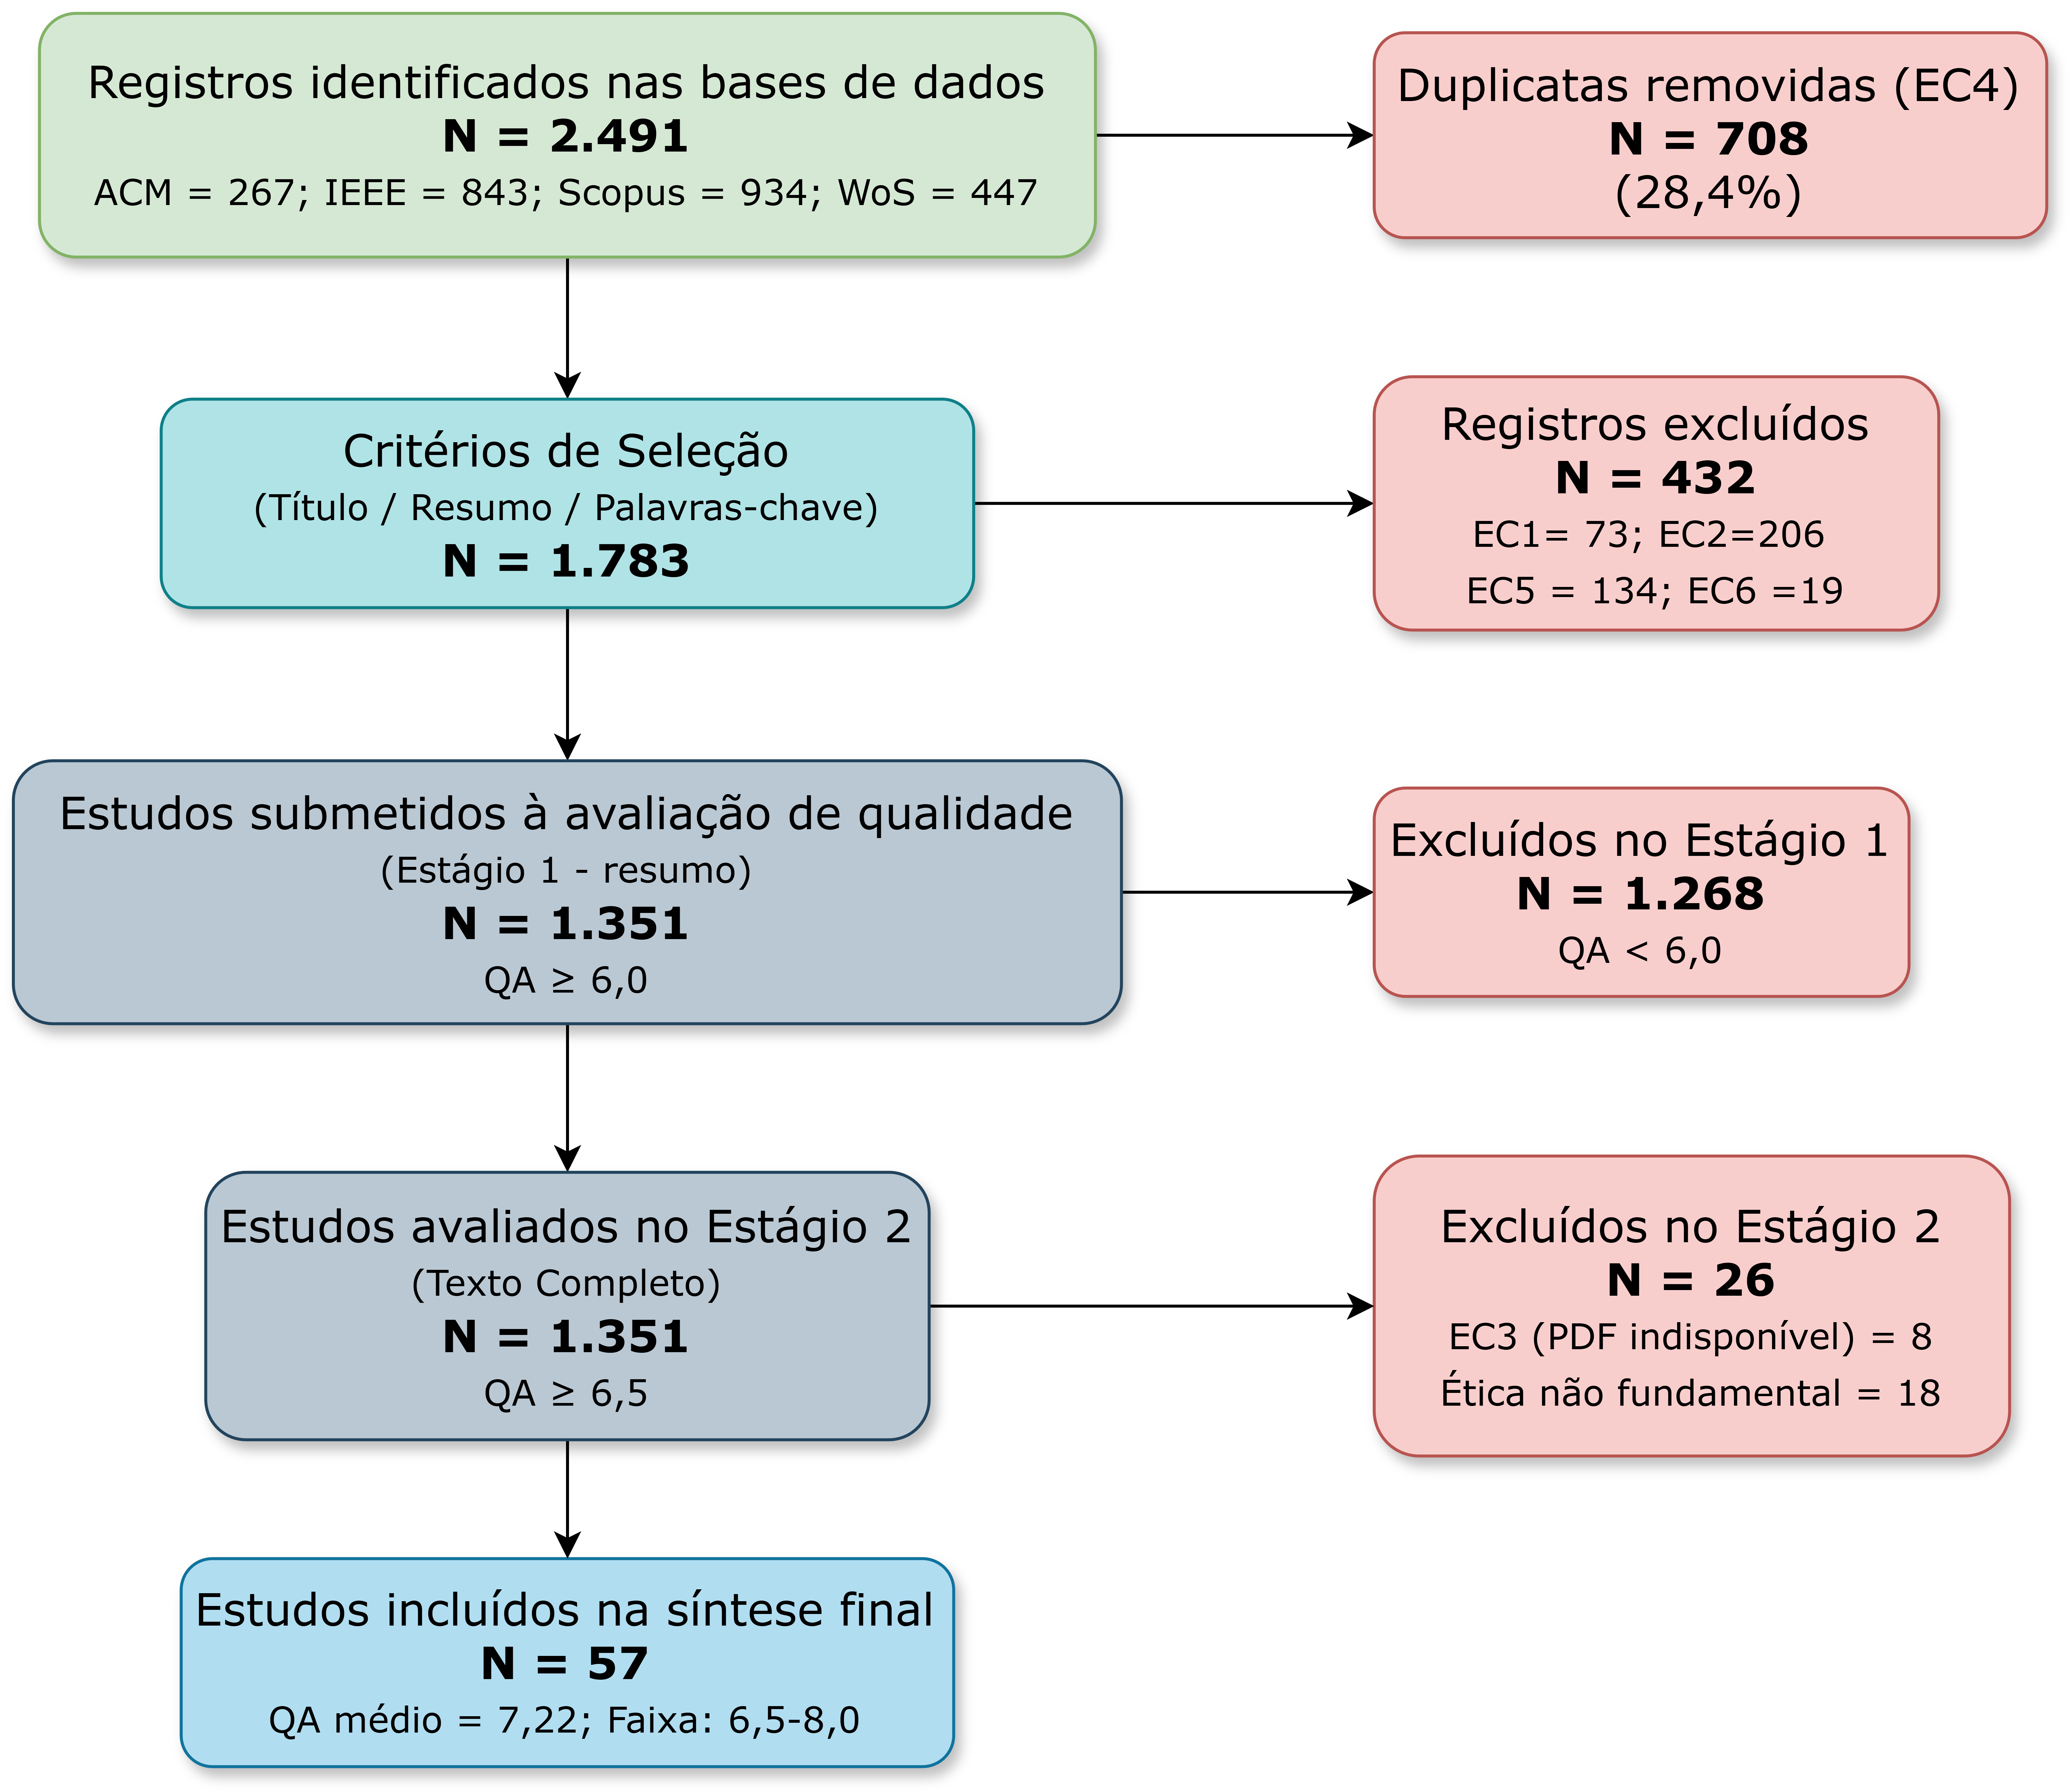
\includegraphics[width=0.75\linewidth]{img/PRISMA2020.png}
    \caption{Fluxograma PRISMA 2020 do processo de identificação, triagem, elegibilidade, avaliação de qualidade e inclusão de estudos.}
    \label{fig:slr}
\end{figure}


As buscas, realizadas em outubro de 2025, resultaram em 2.491 registros iniciais. Após remoção de 708 duplicatas (28,4\%), restaram 1.783 registros para a triagem inicial. Destes, 432 estudos foram descartados por não atenderem aos critérios básicos, resultando em 1.351 artigos submetidos à avaliação de qualidade com base nos critérios de inclusão e exclusão.
A aplicação dos critérios de qualidade aprovou 1.351 estudos para o Estágio 2, enquanto 1.268 foram excluídos no Estágio 1 por não atingirem QA $\geq$ 6,0. No Estágio 2, 26 estudos foram excluídos: 8 por PDF indisponível (EC3) e 18 por ética não fundamental. A análise dos 432 registros excluídos na fase de seleção inicial mostra: EC1 = 73 estudos, EC2 = 206 estudos, EC5 = 134 estudos, e EC6 = 19 estudos. Ao final, 57 estudos foram incluídos na síntese final, com QA médio de 7,22 (faixa: 6,5-8,0).

Dos 1.351 estudos aprovados na triagem IC/EC, 83 foram pré-selecionados no Estágio 1 da Avaliação de Qualidade (análise preliminar com base em abstract, QA $\geq$ 6,0). Esse resultado implica uma taxa de reprovação de 93,9\% (1.268 estudos com QA < 6,0), destacando a elevada disparidade entre a produção científica inicial e os trabalhos que, de fato, atendem aos requisitos mínimos de robustez metodológica e aderência temática. 

No Estágio 2, correspondente à leitura completa dos 83 textos pré-selecionados, constatou-se que 8 estudos permaneciam indisponíveis em texto integral, apesar de tentativas reiteradas de obtenção por meio de contato direto com autores, repositórios institucionais e bibliotecas especializadas. Além disso, 18 estudos foram excluídos após a leitura integral, uma vez que não tratavam a dimensão ética como elemento estruturante da pesquisa, abordando-a apenas de modo tangencial ou restrito a seções acessórias de discussão, o que inviabilizou sua permanência no corpus final da revisão.

Os \textbf{57 estudos restantes} foram incluídos na síntese final (QA $\geq$ 6,5). O escore médio de qualidade foi de 7,22 em 8,0 pontos possíveis (DP = 0,40), evidenciando o alto rigor metodológico dos estudos selecionados.

\begin{table}[htbp]
\centering
\caption{Distribuição dos Estudos por Faixa de Qualidade (57 estudos)}
\label{tab:qa_distribution}
\footnotesize
\begin{tabular}{lccc}
\toprule
\textbf{Faixa de QA} & \textbf{N° Estudos} & \textbf{\% do Corpus} & \textbf{QA Médio} \\
\midrule
6,5 -- 7,0 & 34 & 59,65\% & 6,92 \\
7,5 -- 8,0 & 23 & 40,35\% & 7,65 \\
\midrule
\textbf{Total} & \textbf{57} & \textbf{100,0\%} & \textbf{7,22} \\
\bottomrule
\end{tabular}
\end{table}


%%%%%%%%%%%%%%%%%%%%%%%%%%%%%%%%%%%%%%%%%%%%%%%%%%%%%%%%%%%%%%%%%%%%%%%%%%%%%%%%%%%%%

\section{Extração de Dados}\label{sec:data_extraction}

A extração estruturada de dados é um passo importante para a elaboração de sínteses em revisões sistemáticas. Considerando que o objetivo desta revisão é embasar o modelo proposto, foi adotada uma abordagem restritiva de seleção (como demonstrado pelos critérios IC/EC/QA), o que resultou em um corpus focado e de alta qualidade. As categorias de extração estão intimamente relacionadas às perguntas de pesquisa.

A Tabela~\ref{tab:selected} apresenta a distribuição temporal dos estudos selecionados, permitindo acompanhar a evolução da área ao longo do tempo. Observa-se um crescimento expressivo de 300\% entre 2021 e 2025, passando de 6 estudos anuais para 24, o que demonstra o aumento do interesse acadêmico no tema. A Tabela~\ref{tab:source_distribution}, por sua vez, mostra que IEEE Xplore e Scopus concentram 64,9\% dos estudos de alta qualidade, confirmando sua relevância como fontes primárias para pesquisas em Engenharia de Software e ética em IA.

\begin{table}[htbp]
\centering
\caption{Distribuição temporal dos 57 estudos de alta qualidade (QA $\geq$ 6,5)}
\label{tab:selected}
\footnotesize
\begin{tabular}{lccc}
\hline
\textbf{Ano} & \textbf{Estudos} & \textbf{\% do Corpus} & \textbf{QA Médio} \\
\hline
2021 & 6  & 10,5\%  & 7,55 \\
2022 & 5  & 8,8\%   & 6,95 \\
2023 & 10 & 17,5\%  & 7,46 \\
2024 & 12 & 21,1\%  & 7,17 \\
2025 & 24 & 42,1\%  & 7,37 \\
\hline
\textbf{Total} & \textbf{57} & \textbf{100,0\%} & \textbf{7,22} \\
\hline
\multicolumn{4}{l}{\footnotesize Crescimento de 300\% entre 2021 e 2025 (de 6 para 24 artigos/ano).} \\
\end{tabular}
\end{table}

\begin{table}[htbp]
\centering
\caption{Distribuição por fonte bibliográfica (57 estudos de alta qualidade)}
\label{tab:source_distribution}
\footnotesize
\begin{tabular}{lccc}
\hline
\textbf{Fonte} & \textbf{Estudos} & \textbf{\% do Corpus} & \textbf{QA Médio} \\
\hline
IEEE Xplore           & 24 & 42,1\% & 7,50 \\
Scopus                & 13 & 22,8\% & 7,26 \\
ACM Digital Library   & 11 & 19,3\% & 7,45 \\
Web of Science        & 9  & 15,8\% & 7,00 \\
\hline
\textbf{Total} & \textbf{57} & \textbf{100,0\%} & \textbf{7,22} \\
\hline
\multicolumn{4}{l}{\footnotesize IEEE e Scopus concentram 64,9\% dos estudos de alta qualidade.} \\ 
\end{tabular} 
\end{table}

A Tabela~\ref{tab:principles} sintetiza os dados relacionados à RQ.1. Os princípios éticos foram extraídos mantendo-se a terminologia original dos estudos. Transparency e Explainability foram consolidados em uma única categoria devido à sobreposição conceitual e terminológica observada na literatura, onde os termos frequentemente aparecem associados ou são usados de forma intercambiável. Como muitos estudos abordam múltiplos princípios simultaneamente, o número de menções (217) é superior ao número de estudos (57), resultando em uma média de 3,81 princípios por estudo.

\todo[inline]{porque vc só trabalhou com esses 10 principios? por exemplo, VAkkuri trabalha com varios outros no Eccola e ele é sua referencia 20, 21 27 28}




\begin{table}[htbp]
\centering
\caption{Frequência de princípios éticos nos 58 estudos (múltiplos princípios por estudo)}
\label{tab:principles}
\scriptsize
\begin{tabular}{lccp{6.5cm}}
\hline
\textbf{Princípio Ético} & \textbf{Menções} & \textbf{\% Estudos} & \textbf{Estudos} \\
\hline
Transparency                   & 29 & 50,0\% & \cite{S001}, \cite{S002}, \cite{S003}, \cite{S004}, \cite{S006}, \cite{S007}, \cite{S008}, \cite{S011}, \cite{S012}, \cite{S013}, \cite{S014}, \cite{S015}, \cite{S016}, \cite{S023}, \cite{S024}, \cite{S028}, \cite{S029}, \cite{S033}, \cite{S038}, \cite{S039}, \cite{S041}, \cite{S042}, \cite{S043}, \cite{S044}, \cite{S046}, \cite{S047}, \cite{S050}, \cite{S053}, \cite{S058} \\
\hline
Fairness                       & 48 & 82,8\% & \cite{S001}, \cite{S002}, \cite{S003}, \cite{S004}, \cite{S006}, \cite{S007}, \cite{S008}, \cite{S010}, \cite{S012}, \cite{S013}, \cite{S014}, \cite{S015}, \cite{S017}, \cite{S018}, \cite{S019}, \cite{S020}, \cite{S021}, \cite{S022}, \cite{S023}, \cite{S024}, \cite{S025}, \cite{S028}, \cite{S029}, \cite{S030}, \cite{S031}, \cite{S032}, \cite{S033}, \cite{S034}, \cite{S035}, \cite{S036}, \cite{S038}, \cite{S039}, \cite{S040}, \cite{S041}, \cite{S042}, \cite{S044}, \cite{S045}, \cite{S046}, \cite{S047}, \cite{S048}, \cite{S050}, \cite{S052}, \cite{S053}, \cite{S054}, \cite{S055}, \cite{S056}, \cite{S057}, \cite{S058} \\
\hline
Accountability                 & 32 & 55,2\% & \cite{S001}, \cite{S003}, \cite{S004}, \cite{S005}, \cite{S006}, \cite{S009}, \cite{S012}, \cite{S013}, \cite{S014}, \cite{S016}, \cite{S018}, \cite{S019}, \cite{S023}, \cite{S028}, \cite{S029}, \cite{S033}, \cite{S035}, \cite{S038}, \cite{S039}, \cite{S041}, \cite{S042}, \cite{S043}, \cite{S044}, \cite{S046}, \cite{S048}, \cite{S049}, \cite{S050}, \cite{S051}, \cite{S053}, \cite{S055}, \cite{S056}, \cite{S058} \\
\hline
Trustworthiness                & 21 & 36,2\% & \cite{S001}, \cite{S002}, \cite{S006}, \cite{S009}, \cite{S011}, \cite{S012}, \cite{S014}, \cite{S016}, \cite{S023}, \cite{S024}, \cite{S025}, \cite{S027}, \cite{S028}, \cite{S031}, \cite{S033}, \cite{S037}, \cite{S038}, \cite{S039}, \cite{S047}, \cite{S048}, \cite{S053} \\
\hline
Safety                         & 23 & 39,7\% & \cite{S001}, \cite{S005}, \cite{S008}, \cite{S009}, \cite{S014}, \cite{S015}, \cite{S016}, \cite{S023}, \cite{S025}, \cite{S028}, \cite{S029}, \cite{S033}, \cite{S038}, \cite{S039}, \cite{S041}, \cite{S043}, \cite{S044}, \cite{S045}, \cite{S046}, \cite{S047}, \cite{S051}, \cite{S054}, \cite{S058} \\
\hline
Privacy                        & 18 & 31,0\% & \cite{S003}, \cite{S006}, \cite{S009}, \cite{S012}, \cite{S014}, \cite{S025}, \cite{S028}, \cite{S029}, \cite{S031}, \cite{S033}, \cite{S038}, \cite{S039}, \cite{S041}, \cite{S045}, \cite{S046}, \cite{S048}, \cite{S056}, \cite{S058} \\
\hline
Awareness                      & 17 & 29,3\% & \cite{S001}, \cite{S004}, \cite{S012}, \cite{S018}, \cite{S019}, \cite{S021}, \cite{S022}, \cite{S025}, \cite{S027}, \cite{S029}, \cite{S035}, \cite{S037}, \cite{S041}, \cite{S042}, \cite{S046}, \cite{S049}, \cite{S058} \\
\hline
Sustainability                 & 11 & 19,0\% & \cite{S005}, \cite{S023}, \cite{S025}, \cite{S026}, \cite{S028}, \cite{S030}, \cite{S033}, \cite{S038}, \cite{S040}, \cite{S046}, \cite{S051} \\
\hline
Effectiveness                  & 13 & 22,4\% & \cite{S005}, \cite{S008}, \cite{S015}, \cite{S018}, \cite{S022}, \cite{S024}, \cite{S026}, \cite{S034}, \cite{S035}, \cite{S036}, \cite{S045}, \cite{S046}, \cite{S055} \\
\hline
Beneficence                    & 12 & 20,7\% & \cite{S007}, \cite{S012}, \cite{S019}, \cite{S023}, \cite{S028}, \cite{S029}, \cite{S039}, \cite{S041}, \cite{S042}, \cite{S046}, \cite{S047}, \cite{S058} \\
\hline
\textbf{Total Menções} & \textbf{224} & -- & -- \\
\textbf{Média/Estudo} & \textbf{3,86} & -- & -- \\
\hline
\end{tabular}
\end{table}

A Tabela~\ref{tab:sdlc} sintetiza os dados referentes à RQ.2, com foco na cobertura das etapas do SDLC. As fases foram classificadas conforme a taxonomia tradicional e respeitam os termos empregados pelos próprios autores dos estudos analisados. O total de 156 menções distribuídas entre os 57 estudos resulta em uma média de 2,74 fases do SDLC por estudo, indicando que as abordagens tendem a focar em aspectos específicos do ciclo de vida em vez de cobri-lo integralmente.

\begin{table}[htbp]
\centering
\caption{Frequência de fases SDLC nos 57 estudos (múltiplas fases por estudo)}
\label{tab:sdlc}
\scriptsize
\begin{tabular}{lccp{6.5cm}}
\hline
\textbf{Fase SDLC} & \textbf{Menções} & \textbf{\% Estudos} & \textbf{Exemplos de Estudos} \\
\hline
Requirements                   & 29 & 50,9\% & \cite{S001}, \cite{S002}, \cite{S004}, \cite{S005}, \cite{S006}, \cite{S007}, \cite{S011}, \cite{S012}, \cite{S013}, \cite{S014}, \cite{S023}, \cite{S024}, \cite{S025}, \cite{S028}, \cite{S031}, \cite{S035}, \cite{S037}, \cite{S038}, \cite{S039}, \cite{S042}, \cite{S043}, \cite{S044}, \cite{S045}, \cite{S046}, \cite{S047}, \cite{S050}, \cite{S055}, \cite{S056}, \cite{S058} \\
\hline
Design                         & 26 & 45,6\% & \cite{S001}, \cite{S004}, \cite{S005}, \cite{S006}, \cite{S007}, \cite{S008}, \cite{S009}, \cite{S011}, \cite{S012}, \cite{S013}, \cite{S014}, \cite{S017}, \cite{S025}, \cite{S027}, \cite{S031}, \cite{S033}, \cite{S037}, \cite{S038}, \cite{S039}, \cite{S041}, \cite{S043}, \cite{S046}, \cite{S049}, \cite{S050}, \cite{S053}, \cite{S055} \\
\hline
Implementation                 & 28 & 49,1\% & \cite{S001}, \cite{S005}, \cite{S008}, \cite{S009}, \cite{S010}, \cite{S011}, \cite{S012}, \cite{S013}, \cite{S014}, \cite{S015}, \cite{S021}, \cite{S022}, \cite{S025}, \cite{S026}, \cite{S028}, \cite{S033}, \cite{S034}, \cite{S035}, \cite{S036}, \cite{S037}, \cite{S038}, \cite{S039}, \cite{S041}, \cite{S042}, \cite{S046}, \cite{S050}, \cite{S053}, \cite{S055} \\
\hline
Testing                        & 21 & 36,8\% & \cite{S001}, \cite{S003}, \cite{S004}, \cite{S005}, \cite{S008}, \cite{S010}, \cite{S013}, \cite{S014}, \cite{S015}, \cite{S021}, \cite{S022}, \cite{S026}, \cite{S027}, \cite{S034}, \cite{S036}, \cite{S039}, \cite{S045}, \cite{S046}, \cite{S050}, \cite{S052}, \cite{S055} \\
\hline
Deployment                     & 10 & 17,5\% & \cite{S001}, \cite{S003}, \cite{S009}, \cite{S013}, \cite{S014}, \cite{S017}, \cite{S026}, \cite{S038}, \cite{S041}, \cite{S046} \\
\hline
Operation                      &  9 & 15,8\% & \cite{S001}, \cite{S003}, \cite{S005}, \cite{S013}, \cite{S014}, \cite{S027}, \cite{S038}, \cite{S041}, \cite{S045} \\
\hline
Maintenance                    &  8 & 14,0\% & \cite{S001}, \cite{S009}, \cite{S013}, \cite{S014}, \cite{S030}, \cite{S038}, \cite{S041}, \cite{S046} \\
\hline
DevOps/MLOps                   &  7 & 12,3\% & \cite{S008}, \cite{S021}, \cite{S038}, \cite{S040}, \cite{S044}, \cite{S045}, \cite{S057} \\
\hline
Project Management             &  8 & 14,0\% & \cite{S011}, \cite{S022}, \cite{S025}, \cite{S028}, \cite{S035}, \cite{S038}, \cite{S042}, \cite{S046} \\
\hline
Governance                     & 11 & 19,3\% & \cite{S014}, \cite{S016}, \cite{S028}, \cite{S038}, \cite{S039}, \cite{S041}, \cite{S046}, \cite{S049}, \cite{S053}, \cite{S054}, \cite{S055} \\
\hline
\textbf{Total Menções} & \textbf{156} & -- & -- \\
\textbf{Média/Estudo} & \textbf{2,74} & -- & -- \\
\hline
\end{tabular}
\end{table}

As categorias \textbf{Desafios Reportados} e \textbf{Lacunas Identificadas} dão suporte à análise das RQs 3 e 4. Os desafios foram extraídos preservando-se a formulação original, representando obstáculos que afetam negativamente a adoção ou a efetividade das abordagens. A análise cruzada interpretativa permitiu a identificação de lacunas, que sintetizam necessidades não atendidas e discrepâncias entre o estado atual da prática e os ideais normativos e técnicos.

%%%%%%%%%%%%%%%%%%%%%%%%%%%%%%%%%%%%%%%%%%%%%%%%%%%%%%%%%%%%%%%%%%%%%%%%%%%%%%%%%%%%%

\section{Resultados da RSL}

Esta seção apresenta uma síntese analítica estruturada dos achados da \acrshort{RSL}, organizada para responder, de forma sistemática, a cada uma das questões de pesquisa definidas anteriormente. A análise considera tanto as descobertas individuais de cada estudo quanto os padrões emergentes a partir da síntese cruzada, uma vez que diversos trabalhos abordam princípios ou desafios convergentes sob diferentes perspectivas metodológicas, técnicas ou contextuais.

%%%%%%%%%%%%%%%%%%%%%%%%%%%%%%%%%%%%%%%%%%%%%%%%%%%%%%%%%%%%%%%%%%%%%%%%%%%%%%%%%%%%%

\subsection{RQ.1. Princípios Éticos Aplicáveis ao Desenvolvimento de Software com IA}

A análise do corpus de 57 estudos identificou dez princípios éticos predominantes, com um total de 217 menções (média de 3,81 princípios por estudo), conforme apresentado na Tabela~\ref{tab:principles}. A distribuição evidencia que \textit{Fairness} é o princípio mais prevalente (82,5\%), seguido por \textit{Accountability} (54,4\%) e \textit{Transparency} (49,1\%). Esses três princípios formam a base conceitual da maioria das abordagens identificadas, estando presentes em mais da metade do corpus analisado.

A categoria \textit{Fairness} concentra 47 menções (21,7\% do total), refletindo uma preocupação central com a equidade algorítmica e a mitigação de vieses discriminatórios em sistemas de \acrshort{IA} \cite{Mehrabi2021, Chouldechova2017}. Esse princípio manifesta-se por meio de implementações técnicas específicas, como redução de vieses estatísticos, padronização de métricas entre grupos demográficos \cite{Barocas2019, CorbettDavies2018} e auditoria de equidade algorítmica \cite{Raji2020, buolamwini2018gender}.

\textit{Accountability} (31 menções, 14,3\% do total) enfatiza a rastreabilidade das decisões e a atribuição clara de responsabilidades \cite{Diakopoulos2016, Wieringa2020, Binns2018}, sendo fundamental para a governança de sistemas de IA. Já \textit{Transparency} (28 menções, 12,9\%) aparece frequentemente associada à explicabilidade, refletindo uma sobreposição conceitual observada na literatura \cite{Guidotti2018, BarredoArrieta2020}, na qual transparência e explicabilidade são tratadas como aspectos complementares de um mesmo imperativo ético: tornar sistemas de \acrshort{IA} inteligíveis para diferentes grupos de \textit{stakeholders} \cite{doshivelez2017, miller2018}.

Os princípios de \textit{Safety} (38,6\%) e \textit{Trustworthiness} (36,8\%) aparecem com frequência significativa, sobretudo em estudos voltados a domínios críticos como saúde \cite{Topol2019, Char2020} e transporte autônomo \cite{Borg2019, Koopman2016}, por meio de práticas de engenharia de confiabilidade \cite{Amodei2016, Huang2020} e análise de risco \cite{Uesato2018}.

O princípio da \textit{Privacy} (29,8\%) recebe atenção considerável, especialmente em estudos voltados à conformidade regulatória com legislações como o GDPR \cite{GDPR2016} e a LGPD \cite{LGPD2018}. Destacam-se técnicas como privacidade diferencial \cite{Abadi2016, Dwork2014} e anonimização de dados \cite{El-Emam2013, Fung2010}.

Princípios como \textit{Awareness} (28,1\%), \textit{Effectiveness} (22,8\%), \textit{Sustainability} (19,3\%) e \textit{Beneficence} (19,3\%) aparecem com menor frequência, mas indicam preocupações emergentes. Observa-se uma sub-representação crítica do princípio de \textit{Sustainability} (apenas 19,3\% dos estudos), apesar de seu reconhecimento crescente em frameworks normativos internacionais \cite{UNESCO2021, EUAIAct2024}. Essa negligência é preocupante, dado o aumento das preocupações com a pegada de carbono de modelos de grande escala \cite{Bender2021, Patterson2021} e com os impactos socioambientais de sistemas autônomos \cite{Crawford2021, Luccioni2023}.

A análise revela que apenas uma minoria dos estudos menciona explicitamente frameworks éticos consolidados, como os \textit{OECD AI Principles} \cite{OECD2019}, a \textit{Recommendation on the Ethics of Artificial Intelligence} da UNESCO \cite{UNESCO2021}, ou o \textit{IEEE Ethically Aligned Design} \cite{IEEE2019}. Esse dado sugere uma possível desconexão entre a pesquisa acadêmica em Engenharia de Software e os esforços internacionais de padronização normativa \cite{Floridi2018, Jobin2019}.

%%%%%%%%%%%%%%%%%%%%%%%%%%%%%%%%%%%%%%%%%%%%%%%%%%%%%%%%%%%%%%%%%%%%%%%%%%%%%%%%%%%%%

\subsection{RQ.2. Abordagens de Operacionalização no Ciclo de Vida}

As contribuições identificadas dividem-se em três categorias principais: métodos e processos estruturados (predominantes), avaliações empíricas e \textit{frameworks} conceituais~\cite{Morley2020, McNamara2018}. Em relação à cobertura do SDLC, observa-se uma distribuição relativamente equilibrada entre as fases iniciais e intermediárias, com concentração em \textit{Requirements} (49,1\%), \textit{Implementation} (49,1\%) e \textit{Design} (45,6\%)~\cite{Bellamy2019, Breck2017}, conforme apresentado na Tabela~\ref{tab:sdlc}.

A fase de \textit{Requirements Engineering} está presente em 49,1\% dos estudos (28 de 57), indicando um reconhecimento crescente da importância de incorporar considerações éticas desde as fases iniciais do desenvolvimento. No entanto, ainda há espaço para expansão dessa cobertura, considerando que requisitos éticos devem fundamentar todas as decisões subsequentes do projeto~\cite{Friedman2013, Umbrello2020}.

As abordagens de \textit{Implementation} (49,1\%) concentram-se principalmente em: bibliotecas de \textit{fairness} algorítmica (AIF360~\cite{Bellamy2019}, Fairlearn~\cite{Bird2020}), estratégias de mitigação de viés~\cite{Kamiran2013, Zemel2013}, métodos de explicabilidade local (LIME~\cite{Ribeiro2016}, SHAP~\cite{Lundberg2017}), arquiteturas de privacidade diferencial~\cite{Abadi2016, McMahan2018} e padrões de \textit{logging} para auditabilidade~\cite{Mitchell2019, Arnold2019}. 

A fase de \textit{Design} (45,6\%) demonstra atenção significativa a decisões arquiteturais que incorporam princípios éticos desde a concepção do sistema, alinhando-se com abordagens de \textit{value-sensitive design}~\cite{Friedman2013, VanWynsberghe2013}.

As abordagens de \textit{Testing} (36,8\%) incluem suítes de testes de \textit{fairness}, \textit{frameworks} de validação de explicabilidade, técnicas de \textit{adversarial testing}, auditoria automatizada de viés e metodologias de avaliação de impacto algorítmico. Embora valiosas, essas abordagens concentram-se na verificação pós-implementação.

As fases posteriores do ciclo de vida apresentam cobertura significativamente menor: \textit{Governance} (19,3\%), \textit{Deployment} (17,5\%), \textit{Operation} (15,8\%), \textit{Maintenance} (14,0\%), \textit{Project Management} (14,0\%) e \textit{DevOps/MLOps} (12,3\%). Essa distribuição indica que, apesar dos avanços, ainda existe uma lacuna crítica na cobertura das fases de manutenção e operação contínua.

Quanto à fase de \textit{Governance} (19,3\%), a cobertura ainda é limitada, considerando que \textit{frameworks} normativos contemporâneos (como o AI Act~\cite{EUAIAct2024}) enfatizam fortemente mecanismos organizacionais de supervisão, definição de papéis, responsabilidades e auditoria contínua~\cite{Raji2020, Metcalf2021}.

A análise de maturidade revela que a maioria dos estudos reporta validação experimental em ambientes controlados; uma minoria apresenta estudos de caso ou pilotos, mas há escassez de estudos que documentem a adoção industrial em sistemas produtivos. A limitação de evidências de transferência para ambientes produtivos representa um desafio crítico para a área.

Apenas uma pequena fração dos estudos propõe ferramentas integradas a IDEs, pipelines de CI/CD ou plataformas de MLOps, indicando que muitos pesquisadores desenvolvem soluções isoladas, sem considerar plenamente o ecossistema de ferramentas existente ou a viabilidade de adoção prática~\cite{Hohman2020, Amershi2019}.

\subsection{RQ.3. Evidências Empíricas sobre Efetividade e Limitações}

A análise metodológica revelou a predominância de validações experimentais conduzidas em ambientes controlados, com limitada generalização para contextos industriais. A síntese dos estudos resultou na identificação de cinco categorias principais de desafios enfrentados pelas abordagens de operacionalização ética:

\textbf{Desafios Conceituais:} Ambiguidade na definição operacional de princípios éticos, especialmente \textit{fairness}~\cite{Verma2018, Binns2020} e \textit{transparency}~\cite{Ananny2018, Felzmann2019}; ausência de consenso sobre métricas e indicadores apropriados; falta de formalização de \textit{trade-offs} entre princípios potencialmente conflitantes~\cite{Selbst2019, Green2019}. Apenas uma minoria dos estudos analisados aborda explicitamente essas tensões. O \textit{trade-off} mais investigado sistematicamente foi entre \textit{fairness} e \textit{accuracy}~\cite{Chouldechova2017, Kleinberg2017}, demonstrando que técnicas de mitigação de viés frequentemente resultam em redução da acurácia dos modelos~\cite{Menon2018, CorbettDavies2018}.

\textbf{Desafios Técnicos:} Complexidade de modelos do tipo \textit{black-box}~\cite{Rudin2019, Lipton2018}; escalabilidade limitada de técnicas de explicabilidade~\cite{Lage2019, Bhatt2020}; dificuldades de integração com ferramentas de desenvolvimento existentes~\cite{Amershi2019, Hohman2020}; limitações nas estratégias de mitigação de viés~\cite{Friedler2021, Kallus2018}. Técnicas amplamente adotadas, como LIME~\cite{Ribeiro2016} e SHAP~\cite{Lundberg2017}, apresentam explicações instáveis~\cite{Alvarez-Melis2018} ou de baixa fidelidade~\cite{Ghorbani2019}, comprometendo sua confiabilidade em aplicações reais.

\textbf{Desafios Organizacionais:} Falta de formação técnica em ética entre profissionais de desenvolvimento~\cite{McNamara2018, Fiesler2020}; pressões por entregas rápidas (\textit{time-to-market})~\cite{Rakova2021, Holstein2019}; resistência cultural interna~\cite{Madaio2020, Moss2021}; ausência de papéis ou estruturas organizacionais voltadas à supervisão ética~\cite{Metcalf2021}. Diversos estudos indicam que desenvolvedores percebem práticas éticas como um \textit{overhead} burocrático sem benefícios mensuráveis concretos~\cite{Vakkuri2020, Shneiderman2020}.

\textbf{Desafios Regulatórios:} Fragmentação normativa entre jurisdições~\cite{Veale2021, Bradford2020}; ausência de padrões técnicos certificáveis~\cite{Krafft2020, Brundage2020}; dificuldades de auditoria~\cite{Costanza-Chock2020}; e lacunas entre requisitos legais abstratos e diretrizes técnicas específicas~\cite{Kaminski2023, Selbst2019}. Embora o AI Act defina obrigações prescritivas~\cite{EUAIAct2024}, fornece orientação limitada quanto à implementação prática nos processos de desenvolvimento~\cite{Veale2021, Ebers2021}.

\textbf{Desafios Metodológicos:} Baixa generalização de experimentos acadêmicos; escassez de estudos longitudinais; dificuldades de replicação devido ao uso de dados proprietários; e viés de publicação que favorece estudos com resultados positivos. A escassez de estudos documentando casos industriais limita a avaliação realista dos custos, benefícios e riscos das abordagens propostas em contextos produtivos.

No que diz respeito às evidências de efetividade, os resultados são variados e frequentemente contraditórios. Estratégias de mitigação de viés demonstram bons resultados em benchmarks controlados, mas podem perder efetividade frente a dados reais com distribuições mais complexas. Técnicas de explicabilidade podem melhorar a compreensão em experimentos acadêmicos, mas sua utilidade percebida por \textit{stakeholders} reais permanece uma questão empírica aberta. \textit{Frameworks} de governança apresentam viabilidade conceitual, porém ainda carecem de evidências robustas sobre sua sustentabilidade em organizações reais.

%%%%%%%%%%%%%%%%%%%%%%%%%%%%%%%%%%%%%%%%%%%%%%%%%%%%%%%%%%%%%%%%%%%%%%%%%%%%%%%%%%%%%

\subsection{RQ.4. Lacunas de Conhecimento e Necessidades Futuras}

A síntese integrativa permitiu a identificação de seis lacunas críticas:

\textbf{L1 -- Integração e Rastreabilidade entre Fases:} Embora 49,1\% dos estudos abordem \textit{Requirements Engineering}, 49,1\% abordem \textit{Implementation} e 45,6\% abordem \textit{Design}, observa-se uma lacuna crítica na integração e rastreabilidade de princípios éticos \textit{entre} essas fases~\cite{Friedman2013, Umbrello2020}. A literatura oferece suporte limitado para: rastreabilidade sistemática entre requisitos éticos e artefatos técnicos ao longo do ciclo de vida~\cite{Cleland-Huang2014}, mecanismos de propagação de decisões éticas entre fases~\cite{Ferrario2020}, validação da consistência ética transversal~\cite{Guizzardi2022}, e gestão de \textit{trade-offs} que emergem durante a transição entre requisitos, design e implementação~\cite{Green2019, Selbst2019}. Adicionalmente, persiste a necessidade de métodos mais robustos para elicitação participativa de requisitos éticos~\cite{Ahmad2018, Hadar2018, Shilton2013} e especificação formal de propriedades éticas verificáveis~\cite{Dennis2016}.

\textbf{L2 -- Suporte Ferramental Integrado:} Apenas uma pequena fração dos estudos propõe ferramentas integradas aos ecossistemas de desenvolvimento~\cite{Hohman2020, Amershi2019}. Desenvolvedores necessitam de soluções acopladas a IDEs, sistemas de controle de versão, pipelines de CI/CD e plataformas de MLOps~\cite{Kreuzberger2023, Shankar2022}, em vez de ferramentas \textit{standalone} com fluxos paralelos. A lacuna abrange: plugins para validação ética em tempo de codificação~\cite{Holstein2019, Weisz2021}, integrações com CI/CD para testes automatizados de \textit{fairness}~\cite{Breck2017, Galhotra2017}, dashboards para monitoramento de \textit{ethical drift}~\cite{Paleyes2022}, e frameworks unificados que integrem bibliotecas existentes~\cite{Bellamy2019, Bird2020}.

\textbf{L3 -- Manutenção e Governança Pós-Implantação:} As fases posteriores do ciclo de vida apresentam cobertura significativamente menor: \textit{Governance} (19,3\%), \textit{Deployment} (17,5\%), \textit{Operation} (15,8\%), \textit{Maintenance} (14,0\%), \textit{Project Management} (14,0\%) e \textit{DevOps/MLOps} (12,3\%)~\cite{Paleyes2022}. Sistemas em produção requerem monitoramento contínuo do \textit{ethical drift}~\cite{Klaise2020}, mecanismos de auditoria retrospectiva~\cite{Raji2019, Mitchell2019}, atualizações que preservem propriedades éticas e estruturas organizacionais de governança sustentáveis~\cite{Metcalf2021, Raji2020}. A literatura concentra-se majoritariamente nas fases iniciais e intermediárias do desenvolvimento, negligenciando parcialmente o ciclo completo pós-implantação~\cite{Lwakatare2019, Polyzotis2017}, onde questões éticas frequentemente emergem ou se agravam devido a mudanças nos dados, no contexto de uso ou em requisitos não antecipados.

\textbf{L4 -- Gap Academia-Indústria:} Há escassez de evidências de adoção industrial documentada em sistemas produtivos~\cite{Rakova2021, Holstein2019, Madaio2020}, indicando uma lacuna significativa entre a pesquisa acadêmica e a prática profissional. Faltam evidências sobre: custos reais de implementação~\cite{Sculley2015}, benefícios observáveis e mensuráveis~\cite{Amershi2019}, riscos e falhas em contextos reais~\cite{Piorkowski2021}, barreiras organizacionais e culturais~\cite{Metcalf2021, Moss2021}, e estudos longitudinais sobre a sustentabilidade das práticas éticas~\cite{Lwakatare2019}. Sem tais evidências empíricas de contextos industriais, permanece incerto se as abordagens propostas academicamente são plenamente viáveis, escaláveis e sustentáveis em ambientes produtivos, com suas complexidades organizacionais, técnicas e econômicas.

\textbf{L5 -- Formalização e Negociação de Trade-offs:} Apenas uma minoria dos estudos discute explicitamente tensões e conflitos entre princípios éticos~\cite{Selbst2019, Green2019}. Tais \textit{trade-offs} não são problemas resolvíveis apenas por otimização técnica~\cite{Kleinberg2017}, mas requerem negociação participativa entre \textit{stakeholders}~\cite{Shilton2013}, explicitação transparente de valores e prioridades~\cite{Friedman2013}, documentação rastreável de decisões e justificativas~\cite{Mitchell2019}, e mecanismos de revisão contínua~\cite{Raji2020}. A literatura carece de: métodos estruturados para identificação sistemática de conflitos éticos~\cite{CorbettDavies2018}, frameworks e processos de negociação multistakeholder~\cite{Nathan2007}, técnicas padronizadas de documentação para auditoria~\cite{Arnold2019}, ferramentas para análise de sensibilidade e impacto em cenários de incerteza~\cite{Binns2020}, e abordagens para revisitação de \textit{trade-offs} ao longo do ciclo de vida do sistema.

\textbf{L6 -- Sustentabilidade Socioambiental:} Com apenas 19,3\% de menções (11 estudos), o princípio da \textit{Sustainability} está significativamente sub-representado, apesar de sua crescente relevância em normativas internacionais como a Recomendação da UNESCO~\cite{UNESCO2021} e o AI Act da União Europeia~\cite{EUAIAct2024}. Faltam abordagens sistemáticas para: mensuração e mitigação da pegada de carbono de modelos de IA~\cite{Strubell2019, Patterson2021}, análise de impactos sociais e ambientais de longo prazo (como deslocamento laboral~\cite{Crawford2021}, concentração de poder econômico e tecnológico~\cite{Whittaker2021}, e externalidades ambientais), consideração holística do ciclo de vida completo do sistema (desde a extração de recursos até o descarte), e \textit{trade-offs} explícitos entre desempenho computacional e eficiência energética~\cite{Schwartz2020, Bender2021}. Essa lacuna é particularmente preocupante, considerando o crescimento exponencial no tamanho e no consumo energético de modelos de linguagem e visão computacional.

As necessidades futuras apontadas pela literatura incluem: desenvolvimento de abordagens participativas para engenharia de requisitos éticos envolvendo múltiplos \textit{stakeholders}; ferramentas integradas aos fluxos de trabalho existentes e de fácil utilização por desenvolvedores; métricas objetivas, padronizadas e auditáveis para avaliação de propriedades éticas; programas de capacitação de profissionais em ética aplicada à IA; estudos de caso longitudinais em contextos industriais reais; esforços de padronização técnica por organismos reconhecidos internacionalmente; e integração transversal do tema da ética em IA nos currículos de graduação e pós-graduação nas áreas de Computação e Engenharia de Software.

\section{Síntese do Capítulo}

Este capítulo apresentou o protocolo sistemático de condução da \acrshort{RSL} e a síntese analítica dos resultados. Os achados sumarizados encontram-se nas Tabelas~\ref{tab:selected}, \ref{tab:source_distribution}, \ref{tab:principles} e \ref{tab:sdlc}, bem como na Figura~\ref{fig:slr}. A estratégia de busca, aplicada a quatro bases de dados, resultou em 2.491 registros iniciais. Após deduplicação e triagens sistemáticas (título/resumo, critérios de inclusão e exclusão, avaliação de qualidade em dois estágios), foram incluídos na síntese final \textbf{57 estudos de alta qualidade} (QA $\geq$ 6,5, com QA médio de 7,22).

Os estudos analisados evidenciam um esforço científico significativo na operacionalização de princípios éticos, com destaque para \textit{Fairness} (82,5\%), \textit{Accountability} (54,4\%) e \textit{Transparency} (49,1\%), que formam uma tríade conceitual central. A análise temporal revela um crescimento expressivo de 300\% entre 2021 e 2025, demonstrando o aumento do interesse acadêmico no tema. IEEE Xplore e Scopus concentram 64,9\% dos estudos de alta qualidade, confirmando sua relevância como fontes primárias.

Em relação ao SDLC, observa-se cobertura significativa das fases de \textit{Requirements} (49,1\%), \textit{Implementation} (49,1\%) e \textit{Design} (45,6\%), indicando reconhecimento da importância de integrar considerações éticas desde as fases iniciais. No entanto, as fases posteriores apresentam cobertura menor: \textit{Governance} (19,3\%), \textit{Deployment} (17,5\%), \textit{Operation} (15,8\%), \textit{Maintenance} (14,0\%) e \textit{DevOps/MLOps} (12,3\%).

As abordagens identificadas demonstram efeitos positivos em ambientes controlados; no entanto, a presença de múltiplas variáveis moderadoras e a escassez de evidências industriais dificultam a generalização dos resultados para contextos produtivos reais. Foram identificadas seis lacunas críticas (L1-L6), com destaque para: a necessidade de maior integração ética nas fases iniciais (L1), ausência de suporte ferramental integrado (L2), cobertura limitada de manutenção e governança pós-implantação (L3), escassez de evidências de adoção industrial (L4), falta de formalização de \textit{trade-offs} (L5) e sub-representação da sustentabilidade socioambiental (L6).

Esses resultados fundamentam empiricamente a necessidade e relevância do modelo apresentado no Capítulo~\ref{cap:proposta}, que busca endereçar, de forma sistemática, as lacunas identificadas por meio da incorporação de princípios éticos desde a fase de Engenharia de Requisitos, com suporte de artefatos operacionalizáveis e cobertura abrangente do ciclo de vida de desenvolvimento de software.
